% !Mode:: "TeX:UTF-8"
%!TEX program = xelatex
\documentclass{gmcmthesis}
\hypersetup{hidelinks}
\usepackage{amsmath,amssymb,bm}
\usepackage{newtxmath}
\usepackage{booktabs}
\usepackage{tabularx}
\usepackage{longtable}
\usepackage{multirow}
\usepackage{array}
\usepackage{enumitem}
\usepackage{float}
\usepackage{graphicx}
\usepackage{subfig}
\usepackage{siunitx}
\usepackage[framemethod=TikZ]{mdframed}
\usepackage[noend]{algpseudocode}
\usepackage{algorithmicx,algorithm}
\usepackage{colortbl}
\usepackage{xcolor}
\graphicspath{{figures/}}
\setmainfont{Times New Roman}
\setsansfont{Times New Roman}
\setmonofont{Consolas}
\setcounter{tocdepth}{3}
\setlength{\parindent}{2em}
\setlength{\parskip}{0.25em}
\renewcommand{\arraystretch}{1.18}
\floatname{algorithm}{算法}
\renewcommand{\algorithmicrequire}{\textbf{输入:}}
\renewcommand{\algorithmicensure}{\textbf{输出:}}
\newcommand{\R}{\mathbb{R}}
\newcommand{\E}{\mathbb{E}}
\newcommand{\M}{\mathcal{M}}
\newcommand{\vect}[1]{\bm{#1}}
\newcommand{\code}[1]{\texttt{#1}}
\newcommand{\bertrevision}{\code{12040acc\allowbreak ade4e8a0\allowbreak f71eabdb\allowbreak 258fecc2\allowbreak e7e948be}}
\newcommand{\loss}{\mathcal{L}}
\newcolumntype{Y}{>{\centering\arraybackslash}X}
\newcolumntype{L}{>{\raggedright\arraybackslash}X}
\title{复杂场景下多模态情感识别的统一时间轴建模、层次融合与可解释预测}
\baominghao{\hspace{6em}待填写}
\schoolname{\hspace{5.8em}待填写}
\membera{\hspace{6em}待填写}
\memberb{\hspace{6em}待填写}
\memberc{\hspace{6em}待填写}
\begin{document}
\maketitle
\begin{abstract}
复杂场景下的情感识别同时受到多模态异步、局部缺失、视频时长不一致和决策不可解释等因素影响。本文围绕“文本—语音—视觉”三模态特征的统一建模，建立了一套从原始媒体、时间对齐、监督预测到证据追踪的可审计数学模型。首先，将每条样本划分为50个公共半开时间窗，使用重叠时长加权积分将不同采样率和不同时间粒度的观测映射到同一时间轴；同时以显式掩码区分真实零值与模态缺失，文本侧使用固定版本的 DistilBERT 对题目提供的 \code{text\_bert} token 进行编码，语音与视觉分别构造74维和35维窗口特征。100条样本的时间窗起点、连续性、终点和掩码一致性均通过审计，音频、视觉有效窗率分别为99.00\%和99.80\%，文本有效窗率为58.68\%。

其次，为避免简单拼接模型在长序列和模态缺失下的性能退化，本文设计三路独立的两层双向GRU时序编码器，在模态内部引入掩码时间注意力，在模态之间引入样本级门控，并通过多层融合网络同时预测三分类情感极性和连续情感强度。最终模型固定使用统一的 \code{text\_bert+aligned\_50} 接口，避免训练阶段和专项测试阶段的文本特征漂移。附件2验证集结果表明，相比固定对齐 baseline，最终模型的 Accuracy 从0.612637提升至0.637363，Macro-F1 从0.588115提升至0.601580，MAE 从0.616443下降至0.612262，Pearson相关系数从0.624582提升至0.629627。两者文本特征版本不同，因而这是相同验证划分上的完整系统比较，不能单独归因于网络结构。最后，本文利用模态消融和50窗反事实遮挡输出主要模态、关键时间窗及视频关键帧，最大影响窗的平均置信度下降为0.010919，随机窗仅为0.001215。

本文的主要贡献在于：建立了可审计的三模态公共时间轴；提出了兼顾性能、缺失鲁棒性与可解释性的层次融合模型；给出了严格区分验证指标、无标签专项推理和对齐局限性的完整报告口径。
\keywords{多模态情感识别\quad 公共时间轴\quad 双向GRU\quad 掩码注意力\quad 模态门控\quad 可解释性}
\end{abstract}
\pagestyle{plain}
\maketoc
\clearpage
\section{问题重述与总体思路}
\subsection{研究背景}
情感识别是人机交互、智能客服、心理状态分析和多媒体内容理解中的重要任务。与仅使用文本的情绪分类不同，真实视频中的情感往往同时表现为语言内容、语音韵律和面部或外观变化。三种模态具有不同的采样机制：文本由转写或token序列决定，语音由波形分帧产生，视觉由视频帧率和解码状态决定。如果将它们简单按数组下标拼接，会把“同一个下标”误认为“同一时刻”，从而造成系统性的时间错配。

本题的困难还来自两个方面。第一，复杂场景中某些片段可能没有有效语音、无法检测到人脸或没有文本支持，缺失并不等价于数值为零；如果不显式建模缺失，模型会把填充值当成真实证据。第二，情感强度是连续量，情感极性是离散类别，二者既相关又不完全相同。只优化分类准确率容易造成强度估计不稳定，只优化回归又可能牺牲类别边界。因此，需要建立共享时序表示和双任务输出。
\subsection{题目要求的数学化表达}
设第 $n$ 条样本对应一个时长为 $T_n$ 的视频及其配套文本与音频。令模态集合为
\begin{equation}
\M=\{t,a,v\}.
\label{eq:modalities}
\end{equation}
其中 $t$、$a$、$v$ 分别表示文本、语音和视觉。对每条样本，已知文本极性标签 $y_n^{(c)}\in\{0,1,2\}$ 与连续强度标签 $y_n^{(r)}\in\R$。模型需要完成三个层次的任务：
\begin{enumerate}[label=(\arabic*)]
\item 将原始三模态观测变换为同一条可核验的公共时间轴；
\item 在附件2上学习情感极性与情感强度，并在缺失模态条件下保持稳定；
\item 对附件4无标签样本给出预测、主要模态和关键局部证据，并明确解释结果的边界。
\end{enumerate}
因此，本文不把“对齐”“预测”“解释”视为三个互相独立的脚本，而是将其组织成一条具有统一接口的管线：原始数据审计 $\rightarrow$ 特征提取 $\rightarrow$ 时间窗映射 $\rightarrow$ 掩码归一化 $\rightarrow$ 层次融合 $\rightarrow$ 反事实解释。
\subsection{总体技术路线}
图~\ref{fig:pipeline} 给出本文完整流程。输入层保留文本、音频、视频的原始来源和样本ID；特征层产生 768 维文本、74 维音频和35维视觉描述符；对齐层将所有局部观测投影到50个公共窗口；模型层先独立建模模态内时序，再学习时间注意力和模态门控；输出层同时生成类别、强度及证据文件。
\begin{figure}[htp]
\centering
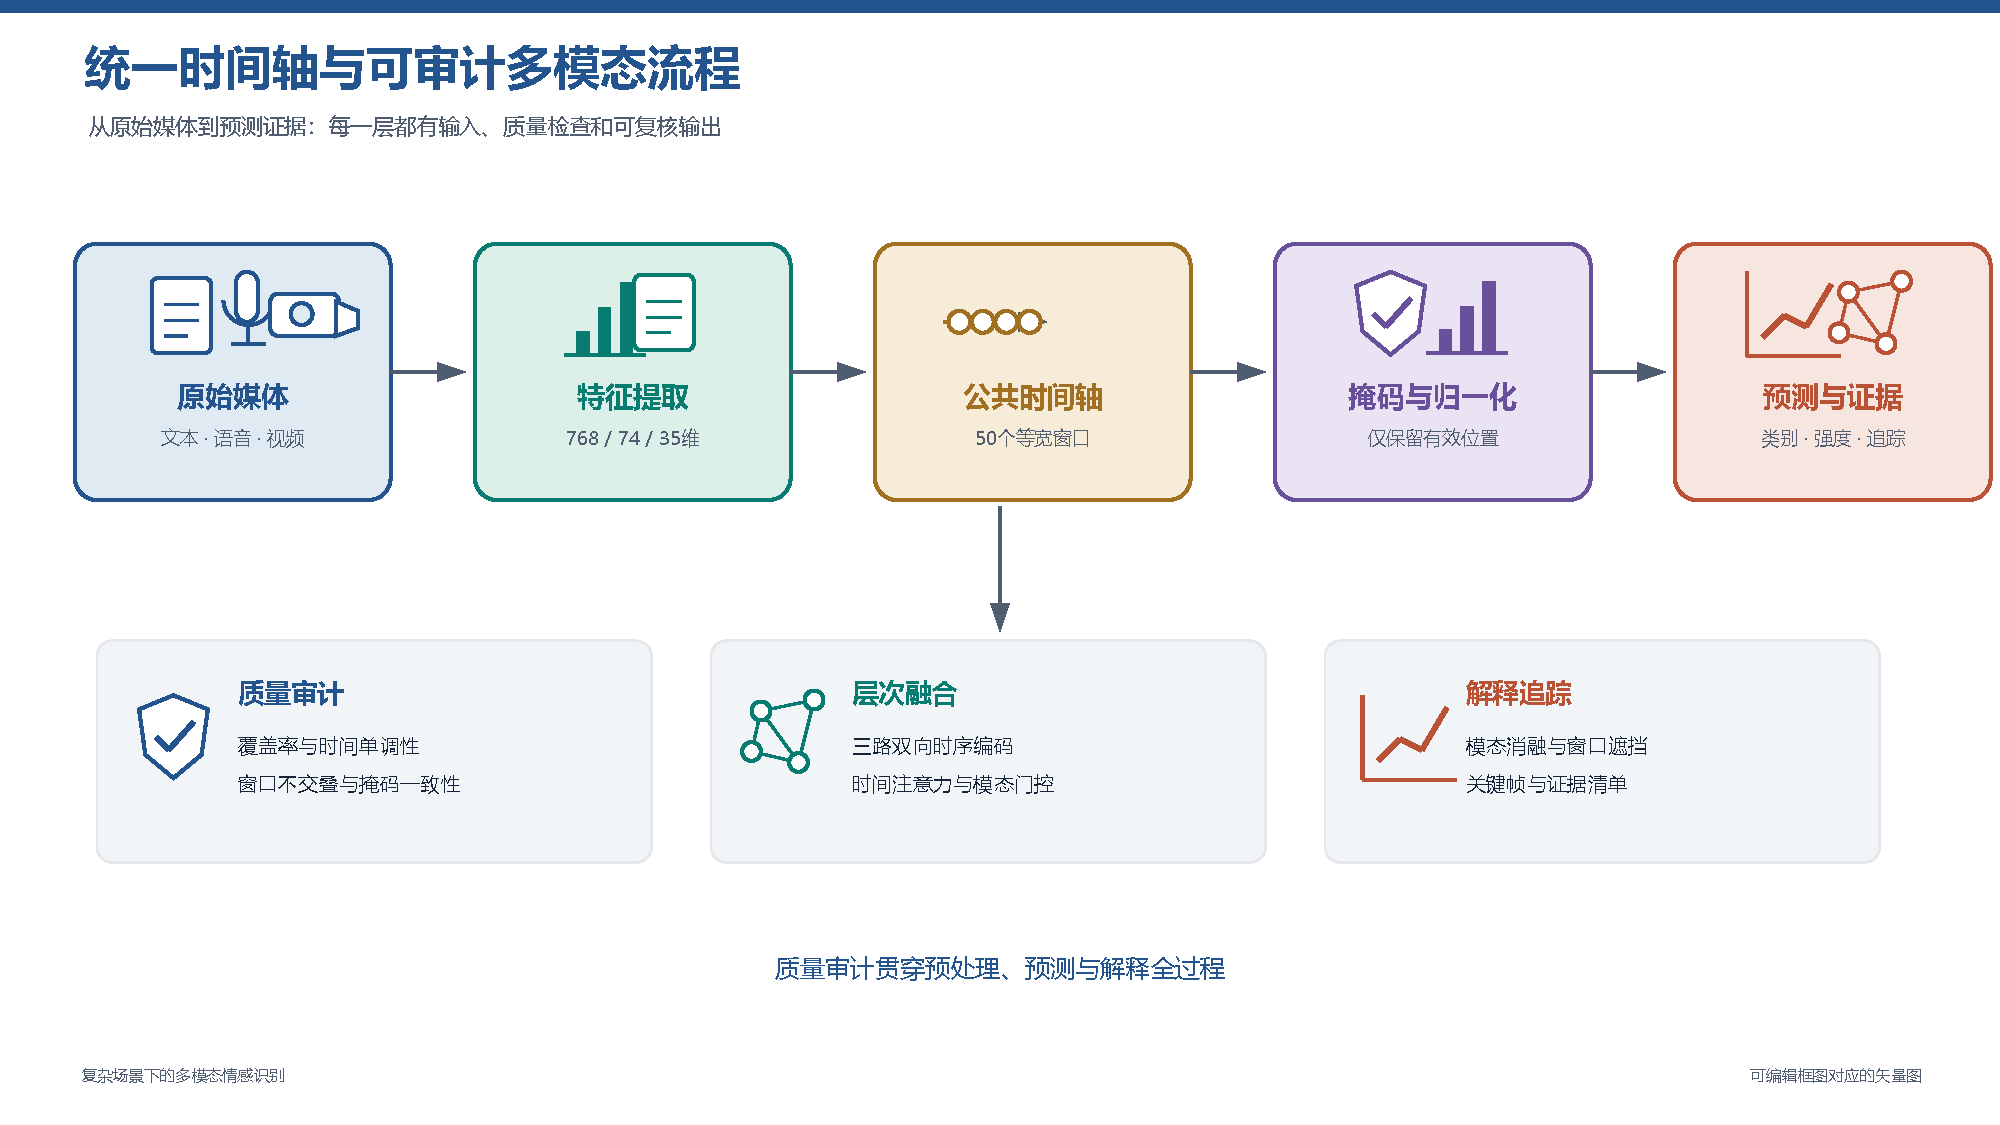
\includegraphics[width=0.98\textwidth]{fig_pipeline}
\caption{三模态情感识别与证据追踪流程}
\label{fig:pipeline}
\end{figure}
与简单 baseline 相比，本文路线的复杂度并非为了堆叠网络，而是服务于三个可验证目标：公共时间窗保证跨模态可比性，掩码机制保证缺失不被误读，注意力和门控机制保证预测能够回溯到模态与时间位置。所有复杂模块都保留对应的消融或反事实验证出口。
\subsection{本文结构与贡献}
本文后续安排如下：第2节给出数据、符号和建模假设；第3节建立公共时间轴和三模态特征提取模型；第4节建立层次化多模态情感预测模型；第5节给出问题2的监督实验、缺失模态测试和附件3推理；第6节给出深入实验、误差剖析与结果解释；第7节给出问题3的可解释预测与证据追踪；第8节讨论敏感性、误差来源、复杂度与推广；第9节总结全文。附录给出数据字典、算法伪代码、完整参数、指标定义、文件清单和可复现命令。
\section{模型假设、符号与评价指标}
\subsection{模型假设}
为保证问题可解并保留可审计性，作如下假设：
\begin{enumerate}[label=\textbf{H\arabic*.}]
\item 每条样本可用一个实际解码得到的媒体时长 $T_n$ 描述，公共窗口均使用半开区间，因此相邻窗口不会重复计算边界点。
\item 音频和视觉的局部观测在其有效时间范围内代表对应窗口的局部状态；媒体末端无真实观测时置为缺失，不使用容器标称长度伪造特征。
\item 文本没有人工词级起止时间戳，因此文本定位只作为弱或半强时间约束；CTC后验、语音活动候选和结构合法性不能替代人工 gold timestamp。
\item 训练集统计量只能由训练划分估计，验证集、附件3和附件4不得反向参与均值、方差、阈值或模型选择。
\item 情感极性和连续强度共享一定的潜在情绪表示，但允许通过两个不同输出头保留任务差异。
\item 模态缺失可以通过掩码被观测，缺失模式本身可能携带信息，因此不对掩码进行随机删除或隐式填零替代。
\end{enumerate}
\subsection{符号说明}
\begin{table}[htp]
\centering
\caption{主要符号及含义}
\label{tab:symbols}
\begin{tabularx}{0.98\textwidth}{cL}
\toprule
符号 & 含义 \\
\midrule
$n$ & 样本索引，$n=1,\ldots,N$ \\
$T_n$ & 第 $n$ 条样本的实际媒体时长 \\
$K$ & 公共时间窗数，本文固定为 $K=50$ \\
$I_{n,k}$ & 第 $n$ 条样本的第 $k$ 个半开时间窗 \\
$m_{n,k}^{(q)}$ & 模态 $q$ 在窗口 $k$ 是否有效的掩码 \\
$z_{n,k}^{(q)}$ & 模态 $q$ 在窗口 $k$ 的归一化特征 \\
$h_{n,k}^{(q)}$ & 模态 $q$ 的时序编码表示 \\
$\alpha_{n,k}^{(q)}$ & 模态 $q$ 内部第 $k$ 个时间窗的注意力权重 \\
$\beta_n^{(q)}$ & 样本级模态门控权重 \\
$\hat y_n^{(c)},\hat y_n^{(r)}$ & 极性预测和强度预测 \\
$\Delta_{n,k}^{(q)}$ & 遮挡一个模态窗口后，目标类别置信度的变化量 \\
\bottomrule
\end{tabularx}
\end{table}
\subsection{评价指标}
分类任务使用 Accuracy 和 Macro-F1。令 $y_i$ 为真实类别、$\hat y_i$ 为预测类别，则
\begin{equation}
\operatorname{Accuracy}=\frac{1}{N}\sum_{i=1}^{N}\mathbb{I}(y_i=\hat y_i).
\label{eq:accuracy}
\end{equation}
对类别 $c$，精确率、召回率和 F1 分数分别为
\begin{equation}
P_c=\frac{TP_c}{TP_c+FP_c},
\label{eq:class_precision}
\end{equation}
\begin{equation}
R_c=\frac{TP_c}{TP_c+FN_c},
\label{eq:class_recall}
\end{equation}
\begin{equation}
F1_c=\frac{2P_cR_c}{P_c+R_c}.
\label{eq:class_f1}
\end{equation}
Macro-F1 为三个类别 F1 的算术平均。由于类别分布可能不均衡，本文将 Macro-F1 作为主分类选择指标，同时报告 Accuracy。
连续情感强度采用平均绝对误差和 Pearson 相关系数：
\begin{equation}
\operatorname{MAE}=\frac{1}{N}\sum_i|y_i^{(r)}-\hat y_i^{(r)}|.
\label{eq:mae}
\end{equation}
\begin{equation}
\rho=\frac{\sum_i(y_i^{(r)}-\bar y)(\hat y_i^{(r)}-\bar{\hat y})}{\sqrt{\sum_i(y_i^{(r)}-\bar y)^2}\sqrt{\sum_i(\hat y_i^{(r)}-\bar{\hat y})^2}}.
\label{eq:pearson}
\end{equation}
对于对齐质量，本文报告覆盖率、时间窗起点为零率、连续率、终点一致率、词段越界率、正时长率、单调率和无重叠率。解释质量不写成因果准确率，而使用最大注意力窗口与随机窗口遮挡后的置信度下降差值
\begin{equation}
\operatorname{TopRandom}=\overline{\Delta}_{\mathrm{top}}-\overline{\Delta}_{\mathrm{random}}.
\label{eq:top_random}
\end{equation}
\clearpage
\section{数据审计与三模态公共时间轴}
\subsection{数据组成与任务划分}
本项目以题目提供的附件2、附件3和附件4为主体，并保留每条样本的原始ID、文本、音频、视频和标签关系。附件2用于训练、验证和独立测试复核；附件3用于缺失模态专项推理，没有真实标签；附件4用于最终预测、证据和视频关键帧回溯，同样没有监督标签。本文所有模型选择只使用附件2训练与验证划分，不使用附件3或附件4的伪标签。
附件2的三模态张量在统一时间窗后形状分别为 $(100,50,768)$、$(100,50,74)$ 和 $(100,50,35)$。文本的768维特征来自固定版本的 \code{distilbert-base-uncased}，具体做法是取最后四层隐状态逐元素均值，并对无效token置零。语音特征以16 kHz单声道解码结果为输入，视觉特征以视频窗口中心附近的真实帧为输入。
\begin{table}[htp]
\centering
\caption{三模态输入与时间定位规则}
\label{tab:modalities}
\begin{tabularx}{0.98\textwidth}{l c L L}
\toprule
模态 & 维度 & 特征构成 & 时间定位与缺失规则 \\
\midrule
文本 & 768 & DistilBERT最后四层均值 & 由题目转写、CTC路径和语音活动候选形成弱或半强定位；低置信或冲突样本屏蔽 \\
语音 & 74 & MFCC、Chroma、谱统计、基频、过零率和RMS & 16 kHz单声道音频分帧，按窗口重叠时长加权；无真实解码覆盖则置掩码0 \\
视觉 & 35 & 人脸、亮度/颜色、纹理、梯度、运动与对称性 & 每窗取最接近中心的真实视频帧；无法解码的窗口置掩码0 \\
\bottomrule
\end{tabularx}
\end{table}
\subsection{公共时间窗模型}
令第 $n$ 条样本实际媒体时长为 $T_n$，固定划分 $K=50$ 个半开公共窗口：
\begin{equation}
I_{n,k}=\left[\frac{kT_n}{K},\frac{(k+1)T_n}{K}\right),\qquad k=0,1,\ldots,K-1.
\label{eq:window}
\end{equation}
半开区间具有两个优点：一方面首窗从0开始，末窗终点严格等于媒体时长；另一方面相邻窗口边界不重复。对于模态 $q$ 的第 $i$ 个局部观测，记其覆盖区间为 $J_{n,i}^{(q)}$，特征为 $x_{n,i}^{(q)}$，则窗口级特征定义为
\begin{equation}
z_{n,k}^{(q)}=\frac{\sum_i |I_{n,k}\cap J_{n,i}^{(q)}|x_{n,i}^{(q)}}{\sum_i |I_{n,k}\cap J_{n,i}^{(q)}|},\quad \text{when }\sum_i |I_{n,k}\cap J_{n,i}^{(q)}|>0.
\label{eq:weighted_pool}
\end{equation}
若分母为零，则令 $z_{n,k}^{(q)}=0$，同时定义 $m_{n,k}^{(q)}=0$。如果窗口内有至少一个有效观测，则 $m_{n,k}^{(q)}=1$。在后续网络中，特征值和掩码始终成对传递，不允许仅凭数值判断窗口是否缺失。
\subsection{文本特征与弱时间约束}
题目提供了两种文本接口：预计算的 \code{text} 和 token 形式的 \code{text\_bert}。为了避免训练和专项测试接口不一致，最终路线固定采用 \code{text\_bert}。对于每个窗口的token集合 $S_{n,k}$，DistilBERT产生最后四层隐状态 $H^{(1)},\ldots,H^{(4)}$，文本表示为
\begin{equation}
z_{n,k}^{(t)}=\frac{1}{|S_{n,k}|}\sum_{j\in S_{n,k}}\frac{1}{4}\sum_{r=1}^{4}H_{n,j}^{(r)}.
\label{eq:text}
\end{equation}
由于没有人工词级起止时间戳，本文不宣称获得 gold 词边界。实际实现采用单调词序分配与CTC后验筛选：先按词元长度和标点停顿构造相对时长，再将其累计映射到视频时长；对存在声学候选的片段保留CTC路径，平均后验低于0.50的样本不进入文本有效窗口。此处的“对齐”指可复现的弱或半强约束，而不是人工验证级强制对齐。
\subsection{语音特征}
音频先由PyAV转换为16 kHz、单声道浮点PCM。每个公共窗口内部使用25 ms帧长、10 ms帧移和512点FFT。74维描述符由以下部分组成：
\begin{enumerate}[label=(\alph*)]
\item 20维MFCC的均值和标准差，共40维，用于表征谱包络与发音差异；
\item 12维Chroma的均值，共12维，用于捕捉音高类别和和声结构；
\item 频谱质心、带宽、滚降点、平坦度、谱熵、谱通量、低频能量比和高频能量比的均值与标准差，共16维；
\item 70--400 Hz谱峰基频的均值和标准差，共2维；
\item 过零率和RMS能量的均值和标准差，共4维。
\end{enumerate}
语音特征既包含相对稳定的谱结构，也包含表达情绪时常见的能量、音高和发声变化。对于音频末端未被真实解码覆盖的窗口，保留窗口位置但令掩码为0。这一处理使模型可区分“低能量但存在的声音”与“根本没有有效音频”。
\subsection{视觉特征}
视觉特征从窗口中心附近真实帧提取。首先将视频帧缩放至宽度不超过320像素，随后使用传统人脸检测获取人脸存在性和归一化框几何；同时计算全帧亮度、HSV颜色、边缘、梯度、拉普拉斯和图像熵等统计；最后通过相邻窗口或稠密光流构造运动量。35维特征的组成见表~\ref{tab:vision_features}。
\begin{table}[htp]
\centering
\caption{35维视觉特征构成}
\label{tab:vision_features}
\begin{tabularx}{0.95\textwidth}{c L c}
\toprule
组别 & 描述 & 维数 \\
\midrule
人脸 & 存在性、归一化中心、宽高、面积比例等 & 6 \\
全帧外观 & 亮度统计、HSV颜色统计 & 12 \\
纹理与边缘 & 边缘、梯度、拉普拉斯响应和图像熵 & 5 \\
运动 & 稠密光流的水平、垂直、幅值及稳定性 & 4 \\
局部结构 & 人脸或中心区域亮度、左右对称性与局部差异 & 8 \\
\bottomrule
\end{tabularx}
\end{table}
视觉没有检测到人脸不等价于视觉模态缺失，因为背景亮度、运动和颜色仍可能对情感判断有贡献。因此仅将人脸相关特征置为相应值，只有无法解码真实帧时才将整个视觉窗口掩码为0。
\subsection{对齐质量审计}
最终输出包含5000个公共窗口。时间结构核验显示，100\%样本的第一个窗口从0开始，100\%样本的窗口连续，100\%样本的最后一个窗口终点等于媒体实际时长，窗口正时长率为100\%。词级记录共有1629条，边界越界率、非正时长率、非单调率和重叠率均为0。
模态覆盖率如图~\ref{fig:alignment_quality} 所示。语音有效窗率99.00\%，视觉有效窗率99.80\%，文本有效窗率58.68\%，反映转写、声学支持与保守屏蔽规则共同造成的缺失。文本缺失被显式保留并由模型掩码处理，而不是被错误填成全程有效。
\begin{figure}[htp]
\centering
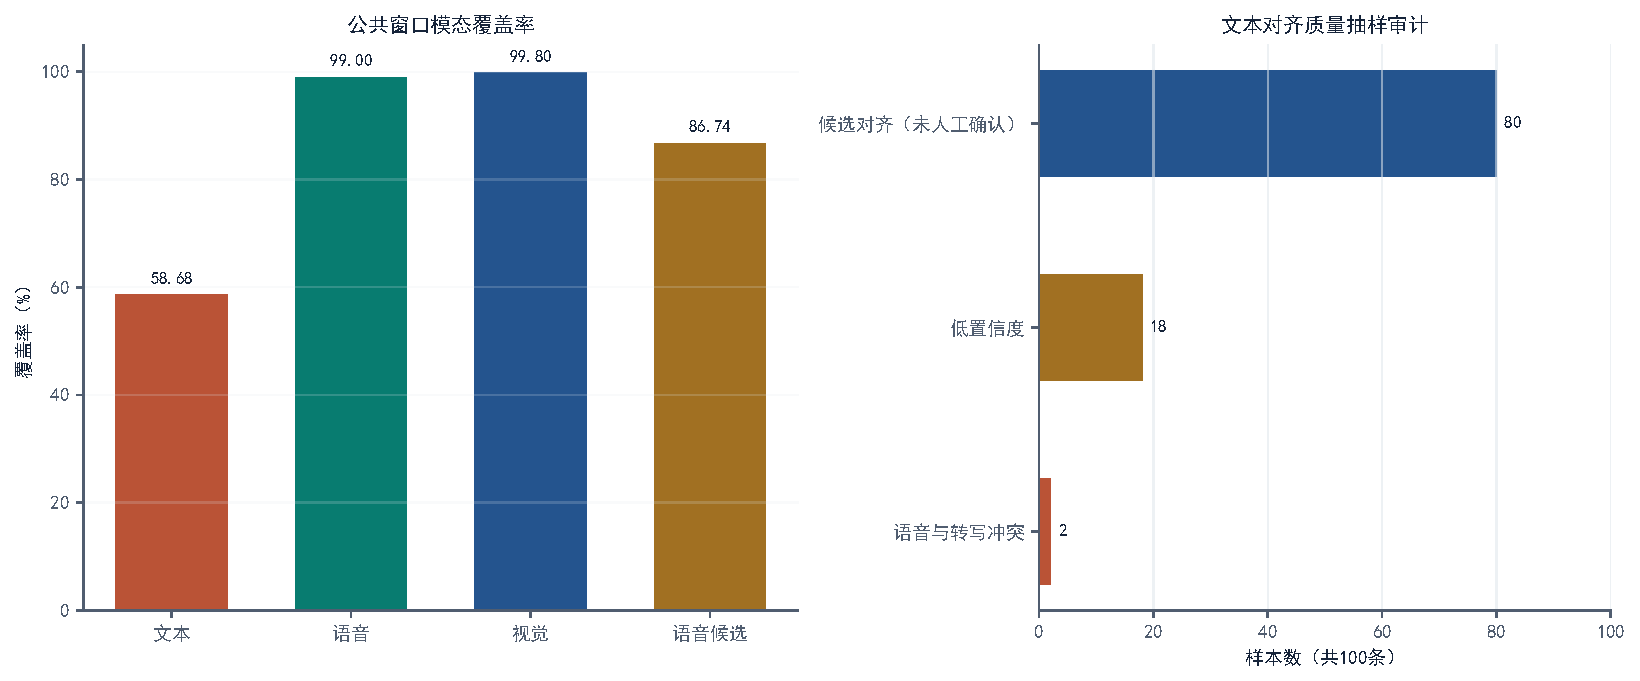
\includegraphics[width=0.95\textwidth]{fig_alignment_quality}
\caption{公共时间窗覆盖率与文本对齐审计}
\label{fig:alignment_quality}
\end{figure}
\subsection{典型样本的时间轴展示}
选取时长接近中位数且音视频覆盖完整的样本进行可视化。该样本时长为6.644987秒，单窗宽度约为0.132900秒。图~\ref{fig:typical_timeline} 上半部分显示50个等宽公共窗口，下半部分展示五个代表窗口中心附近的真实视频帧；窗口色块仅示意边界和顺序，不是模拟的语音信号。为避开视频自带的外文下沿水印，图示视频帧统一裁切下缘约13\%，原始视频帧及证据定位文件均保持不变。此图用于说明“窗口位置”由真实媒体时长决定，而不是由特征数组长度直接猜测。
\begin{figure}[htp]
\centering
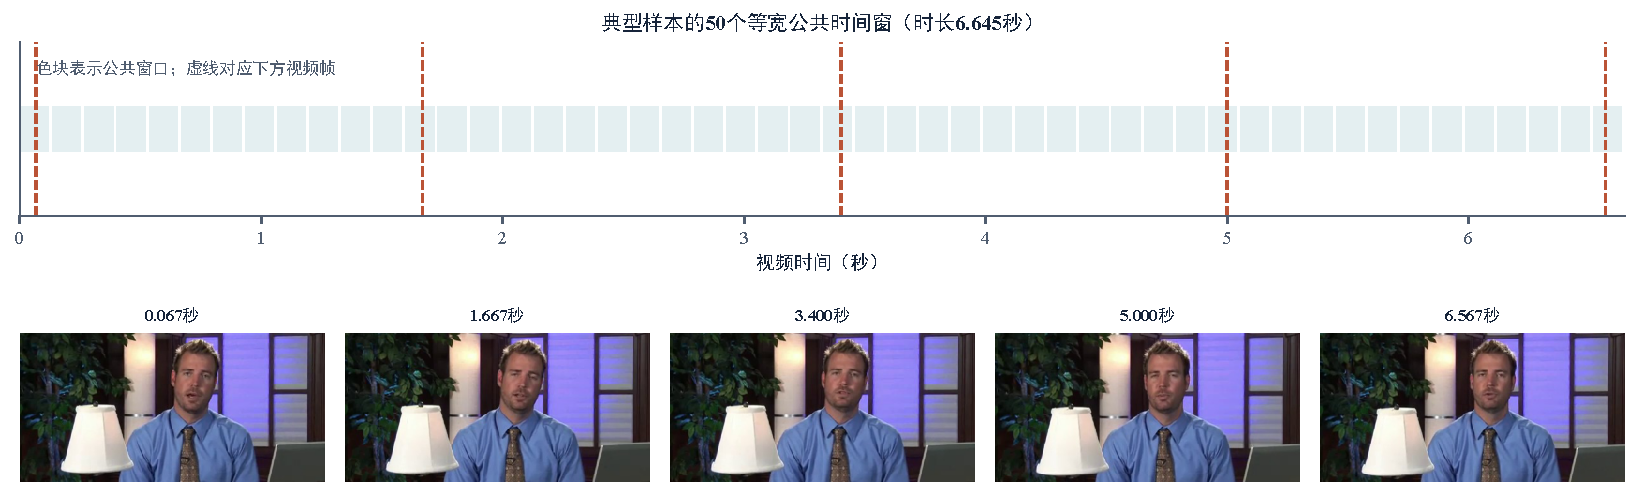
\includegraphics[width=0.96\textwidth]{fig_typical_timeline}
\caption{典型样本的50窗时间轴与视频帧}
\label{fig:typical_timeline}
\end{figure}
\subsection{对齐结果的边界}
本题数据没有人工词级 gold timestamp，因此不能计算词起点MAE、词终点MAE、±10/20/50 ms命中率或词区间IoU。CTC后验均值0.912124和中位数0.982779是模型内部置信信号，不是人工准确率。本文将这些数值用于质量审计，不把它们写成对齐准确率。对后续研究而言，随机抽取约20条样本进行人工词边界标注，就可以把现有结构指标升级为真实的边界误差评价。
clearpage
\section{层次化多模态情感预测模型}
\subsection{简单 baseline 与设计动机}
固定对齐 baseline 将三个模态在50个窗口上的统计表示直接输入浅层融合网络，用于建立“已有特征是否本身可用”的参照。它的优点是参数少、训练快、易于复现；不足是无法区分模态内部不同时间窗的重要性，也不能自然地表示模态缺失。本文设计复杂主模型的目标不是盲目增加参数，而是逐层回答三个问题：哪个模态在当前样本中更有用、哪个时间窗贡献更大、情感类别和强度如何共享信息。
\subsection{掩码归一化}
设训练集统计量为 $\mu^{(q)},\sigma^{(q)}$，则模态 $q$ 的归一化特征为
\begin{equation}
\tilde z_{n,k}^{(q)}=m_{n,k}^{(q)}\cdot\operatorname{clip}\left(\frac{z_{n,k}^{(q)}-\mu^{(q)}}{\sigma^{(q)}},-10,10\right).
\label{eq:normalize}
\end{equation}
其中 $\mu^{(q)}$ 与 $\sigma^{(q)}$ 只由训练集有效窗口计算。式~\eqref{eq:normalize} 的关键是先归一化再乘mask，避免缺失窗口影响统计量；同时保留 $m_{n,k}^{(q)}$ 作为网络输入。
\subsection{模态内时序编码器}
对于模态 $q$，先使用线性投影将原始维度映射到隐藏维度 $d=128$：
\begin{equation}
e_{n,k}^{(q)}=\operatorname{GELU}(W_q\tilde z_{n,k}^{(q)}+b_q)\odot m_{n,k}^{(q)}.
\end{equation}
随后使用两层双向GRU。对正向和反向隐藏状态分别记为 $\overrightarrow h_{n,k}^{(q)}$ 与 $\overleftarrow h_{n,k}^{(q)}$，拼接后得到
\begin{equation}
h_{n,k}^{(q)}=\operatorname{LayerNorm}\left(e_{n,k}^{(q)}+\operatorname{Dropout}\left([\overrightarrow h_{n,k}^{(q)};\overleftarrow h_{n,k}^{(q)}]\right)\right)\odot m_{n,k}^{(q)}.
\label{eq:bigru}
\end{equation}
双向结构能够同时利用窗口前后的局部变化，对短视频中“先铺垫后转折”的情绪表达尤其重要；残差加法使投影后的瞬时特征不会被循环状态完全覆盖。
\subsection{模态内时间注意力}
对每个模态使用一个线性评分器得到窗口得分
\begin{equation}
s_{n,k}^{(q)}=w_q^{\top}\operatorname{LayerNorm}(h_{n,k}^{(q)})+b_q.
\end{equation}
对掩码为0的位置施加负无穷屏蔽，并归一化为
\begin{equation}
\alpha_{n,k}^{(q)}=\frac{m_{n,k}^{(q)}\exp(s_{n,k}^{(q)})}{\sum_{j=1}^{K}m_{n,j}^{(q)}\exp(s_{n,j}^{(q)})+\epsilon}.
\end{equation}
模态级池化表示为
\begin{equation}
p_n^{(q)}=\sum_{k=1}^{K}\alpha_{n,k}^{(q)}h_{n,k}^{(q)}.
\label{eq:attention_pool}
\end{equation}
因此 $\alpha$ 既参与预测，也提供局部证据排序的第一层候选。需要强调的是，注意力不是因果解释；本文还会用遮挡实验检验注意力最高位置是否比随机位置更影响预测。
\subsection{样本级模态门控}
将三种模态池化表示拼接为 $p_n=[p_n^{(t)};p_n^{(a)};p_n^{(v)}]$，门控网络输出
\begin{equation}
\vect g_n=W_2\operatorname{GELU}(W_1\operatorname{LayerNorm}(p_n)+b_1)+b_2.
\label{eq:gate_logits}
\end{equation}
\begin{equation}
\beta_n=\operatorname{softmax}(\vect g_n).
\label{eq:gate}
\end{equation}
其中 $\beta_n^{(q)}\ge0$ 且 $\sum_q\beta_n^{(q)}=1$。门控后的融合输入为
\begin{equation}
f_n=[\beta_n^{(t)}p_n^{(t)};\beta_n^{(a)}p_n^{(a)};\beta_n^{(v)}p_n^{(v)}].
\end{equation}
这样，模型可以针对不同样本自适应改变模态作用程度：例如语音缺失时，音频门控可能降低；文本证据完整时，文本门控可能提高。但门控权重仍是模型内部的相对贡献，不等同于人类心理机制。
\subsection{融合层与双任务输出}
融合层采用“线性扩展—GELU—Dropout—线性压缩—LayerNorm”的结构：
\begin{equation}
r_n=\operatorname{GELU}\left(\operatorname{LayerNorm}\left(W_f^{(2)}\operatorname{Dropout}(\operatorname{GELU}(W_f^{(1)}f_n+b_f^{(1)}))+b_f^{(2)}\right)\right).
\end{equation}
分类头与回归头分别为
\begin{equation}
\hat{\vect p}_n=\operatorname{softmax}(W_c r_n+b_c).
\label{eq:class_head}
\end{equation}
\begin{equation}
\hat y_n^{(r)}=W_r r_n+b_r.
\label{eq:regression_head}
\end{equation}
训练损失取交叉熵与Smooth L1回归损失的加权和：
\begin{equation}
\loss=\loss_{\mathrm{CE}}+\lambda_r\loss_{\mathrm{SmoothL1}},\qquad \lambda_r=0.5.
\label{eq:loss}
\end{equation}
最终模型按验证集综合分数 $F1_{macro}-0.1\times MAE$ 选择最优轮次，同时保留Accuracy、Pearson和解释指标供审查。
\subsection{模型流程图与复杂度}
图~\ref{fig:model_arch} 展示了模型结构。每个模态包含一个输入投影、两层双向GRU和时间注意力，三路输出再通过门控和融合层产生两个任务的结果。对长度 $K$、隐藏维度 $d$、模态数 $M=3$ 的输入，三路GRU的时间计算量约为 $O(MKd^2)$，注意力与门控的计算量分别约为 $O(MKd)$ 和 $O(Md^2)$。与简单拼接相比，增加的计算主要用于捕捉时间依赖和模态相对作用，仍远小于端到端视频Transformer的时空注意力复杂度。
\begin{figure}[htp]
\centering
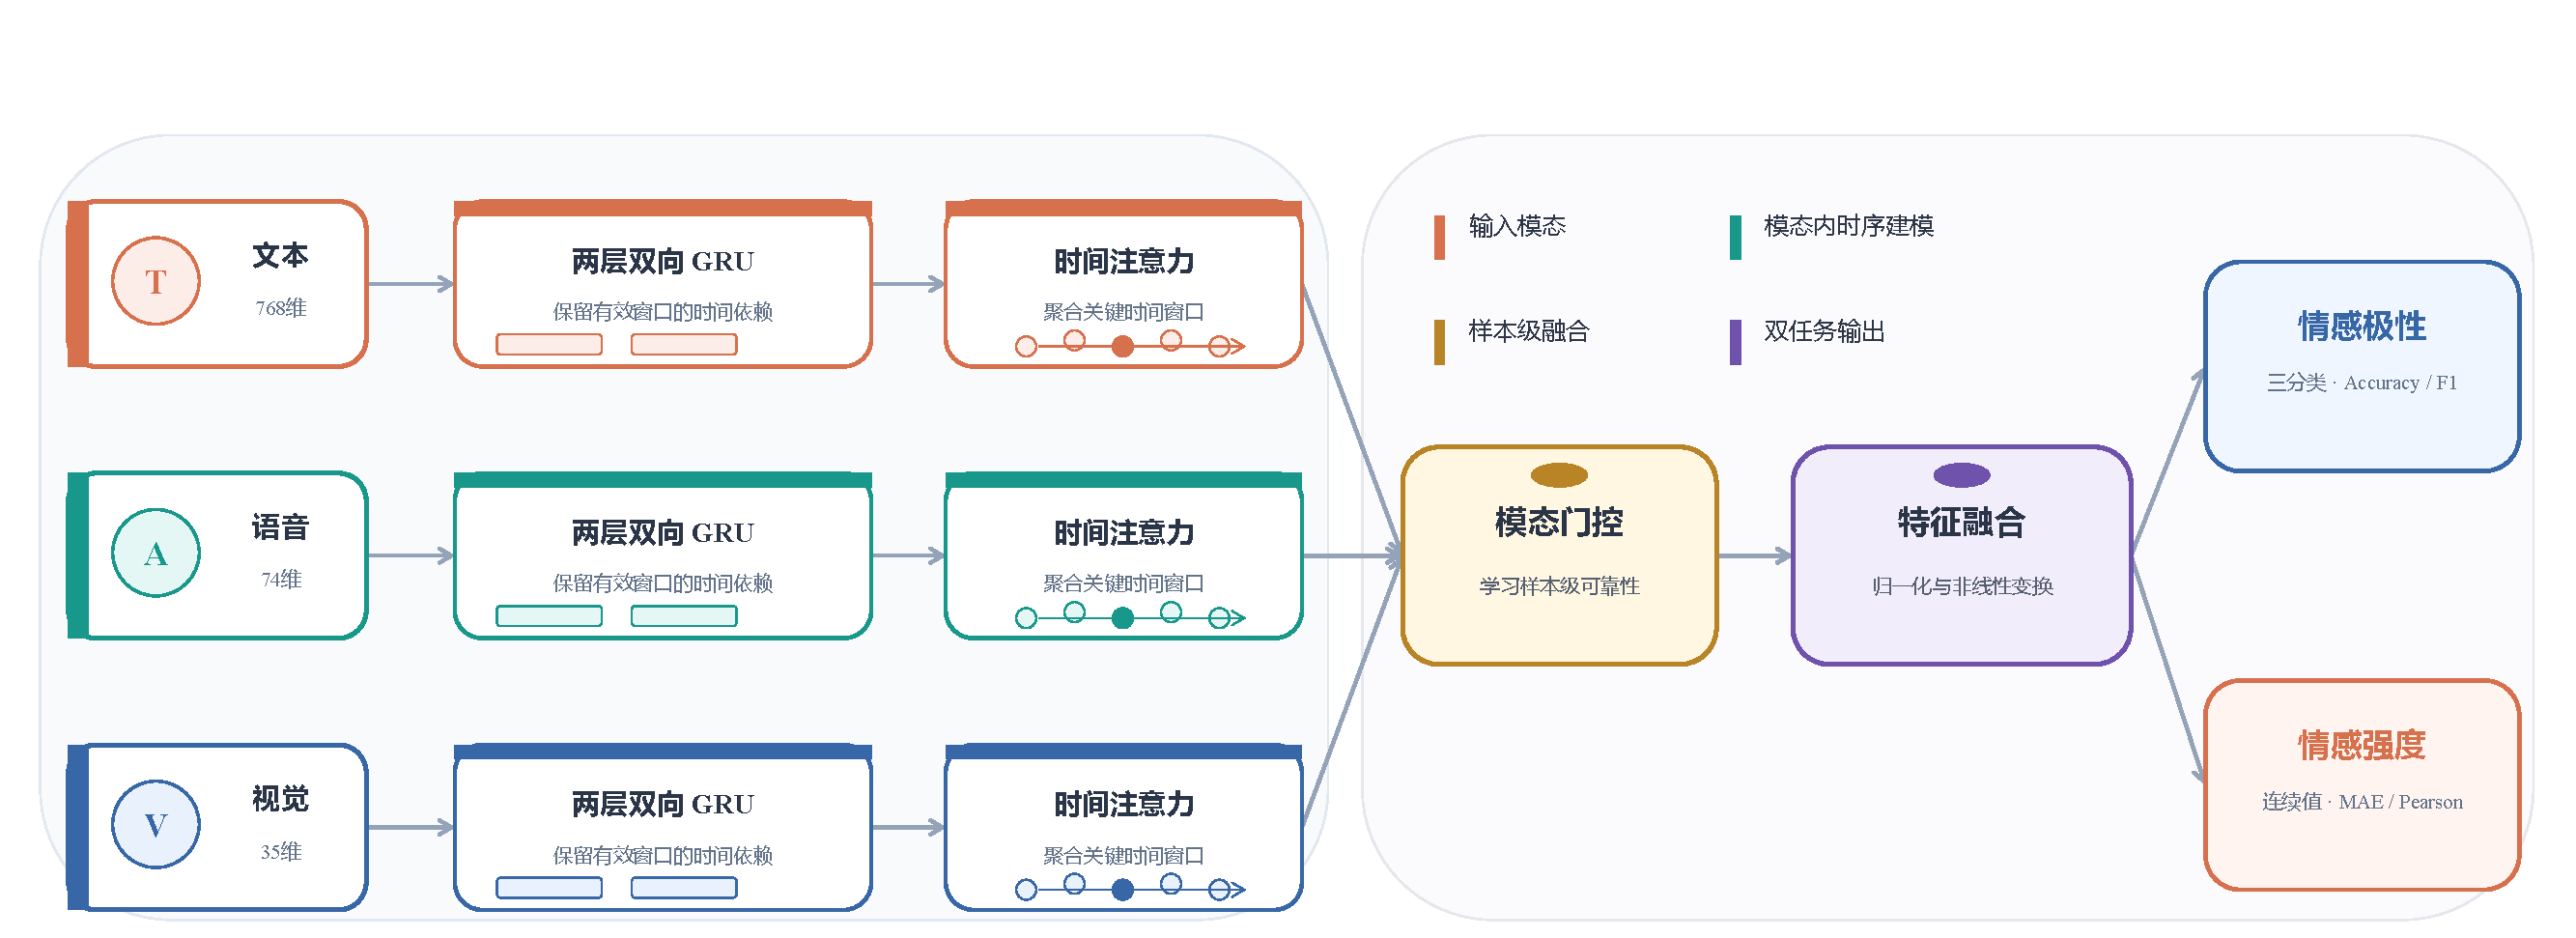
\includegraphics[width=0.98\textwidth]{fig_model_architecture}
\caption{层次化多模态情感预测模型}
\label{fig:model_arch}
\end{figure}
\subsection{训练算法}
算法~\ref{alg:training} 给出训练和验证的核心步骤。特别地，归一化统计量先从训练集计算；模型保存依据验证集，不读取附件3或附件4标签。
\begin{algorithm}[htp]
\caption{统一接口下的层次化多模态双任务训练}
\label{alg:training}
\begin{algorithmic}[1]
\Require 训练集 $D_{tr}$、验证集 $D_{va}$，三模态特征与掩码
\Ensure 最优 checkpoint、验证指标与训练历史
\State 用 $D_{tr}$ 有效窗口计算每个模态的 $\mu^{(q)},\sigma^{(q)}$
\State 对所有样本执行式~\eqref{eq:normalize}，保留 $m^{(q)}$
\State 初始化三路BiGRU、时间注意力、门控、融合层和双任务头
\For{epoch $=1,\ldots,E$}
  \For{mini-batch $B\subset D_{tr}$}
    \State 计算三路编码 $h^{(q)}$ 与掩码注意力 $\alpha^{(q)}$
    \State 计算模态门控 $\beta$、融合表示 $r$ 与两项预测
    \State 按式~\eqref{eq:loss} 计算损失，反向传播并更新参数
  \EndFor
  \State 在 $D_{va}$ 上计算 Accuracy、Macro-F1、MAE、Pearson
  \State 若 $F1_{macro}-0.1MAE$ 提升，则保存当前模型
\EndFor
\State 返回验证分数最高的 checkpoint
\end{algorithmic}
\end{algorithm}
\clearpage
\section{问题二：监督预测与缺失模态测试}
\subsection{实验协议与公平比较}
为了保证比较可解释，本文把固定 aligned baseline、长度感知重采样 baseline、无标签表征融合、双向GRU融合、旧残差融合和统一编码最终模型分开报告。固定 baseline 使用原始 \code{aligned\_features.pkl}，最终模型使用 \code{aligned\_text\_bert\_features.pkl}；两者的附件2验证划分相同，但文本特征并不相同。因此跨模型的四项差异是系统级对比，不是“仅改变网络架构”的控制实验；统一接口的合规性专指最终模型自身训练、验证与专项推理一致。旧残差模型的附件2训练与附件3文本重建使用了不同接口，因此只作为历史指标对照，不作为最终模型。
附件2训练集和验证集只参与监督学习与模型选择，附件2 test 划分只作独立复核；附件3无标签，只输出预测分布和缺失敏感性；附件4无标签，只输出预测及解释证据。任何无标签附件均不用于反向选模。
\subsection{各候选模型比较}
表~\ref{tab:candidates} 汇总候选模型的验证结果。固定 baseline 的回归指标较稳，但缺少显式的时间建模和模态解释；残差融合在旧接口下取得较高Macro-F1；最终统一编码注意力—门控模型在四项报告指标上同时超过固定 baseline，满足“复杂度、合规性和性能”三个条件。
\begin{table}[htp]
\centering
\small
\caption{候选模型在附件2验证集上的结果}
\label{tab:candidates}
\begin{tabular}{lrrrrl}
\toprule
模型 & Accuracy & Macro-F1 & MAE & Pearson & 备注 \\
\midrule
Fixed aligned baseline & 0.612637 & 0.588115 & 0.616443 & 0.624582 & 简单参照 \\
Length-aware resampled baseline & 0.614011 & 0.595798 & 0.614132 & 0.620838 & 数据版本候选 \\
Label-free SSL fusion & 0.608516 & 0.578294 & 0.667391 & 0.573212 & 不选用 \\
Bidirectional SSL fusion & 0.618132 & 0.598285 & 0.621818 & 0.588408 & 对比模型 \\
Old residual fusion & 0.622253 & 0.610330 & 0.623941 & 0.601396 & 接口不合规对照 \\
Final attention-gate model & \textbf{0.637363} & \textbf{0.601580} & \textbf{0.612262} & \textbf{0.629627} & 最终主模型 \\
\bottomrule
\end{tabular}
\end{table}
图~\ref{fig:model_comparison} 将不同候选模型的四项指标分开展示。最终模型的优势不是只体现在一个分类指标：它在Accuracy与Macro-F1上更高，在MAE上更低，在Pearson上更高。这种多指标同时改善比单独追求Accuracy更适合作为双任务模型的主结果。
\begin{figure}[htp]
\centering
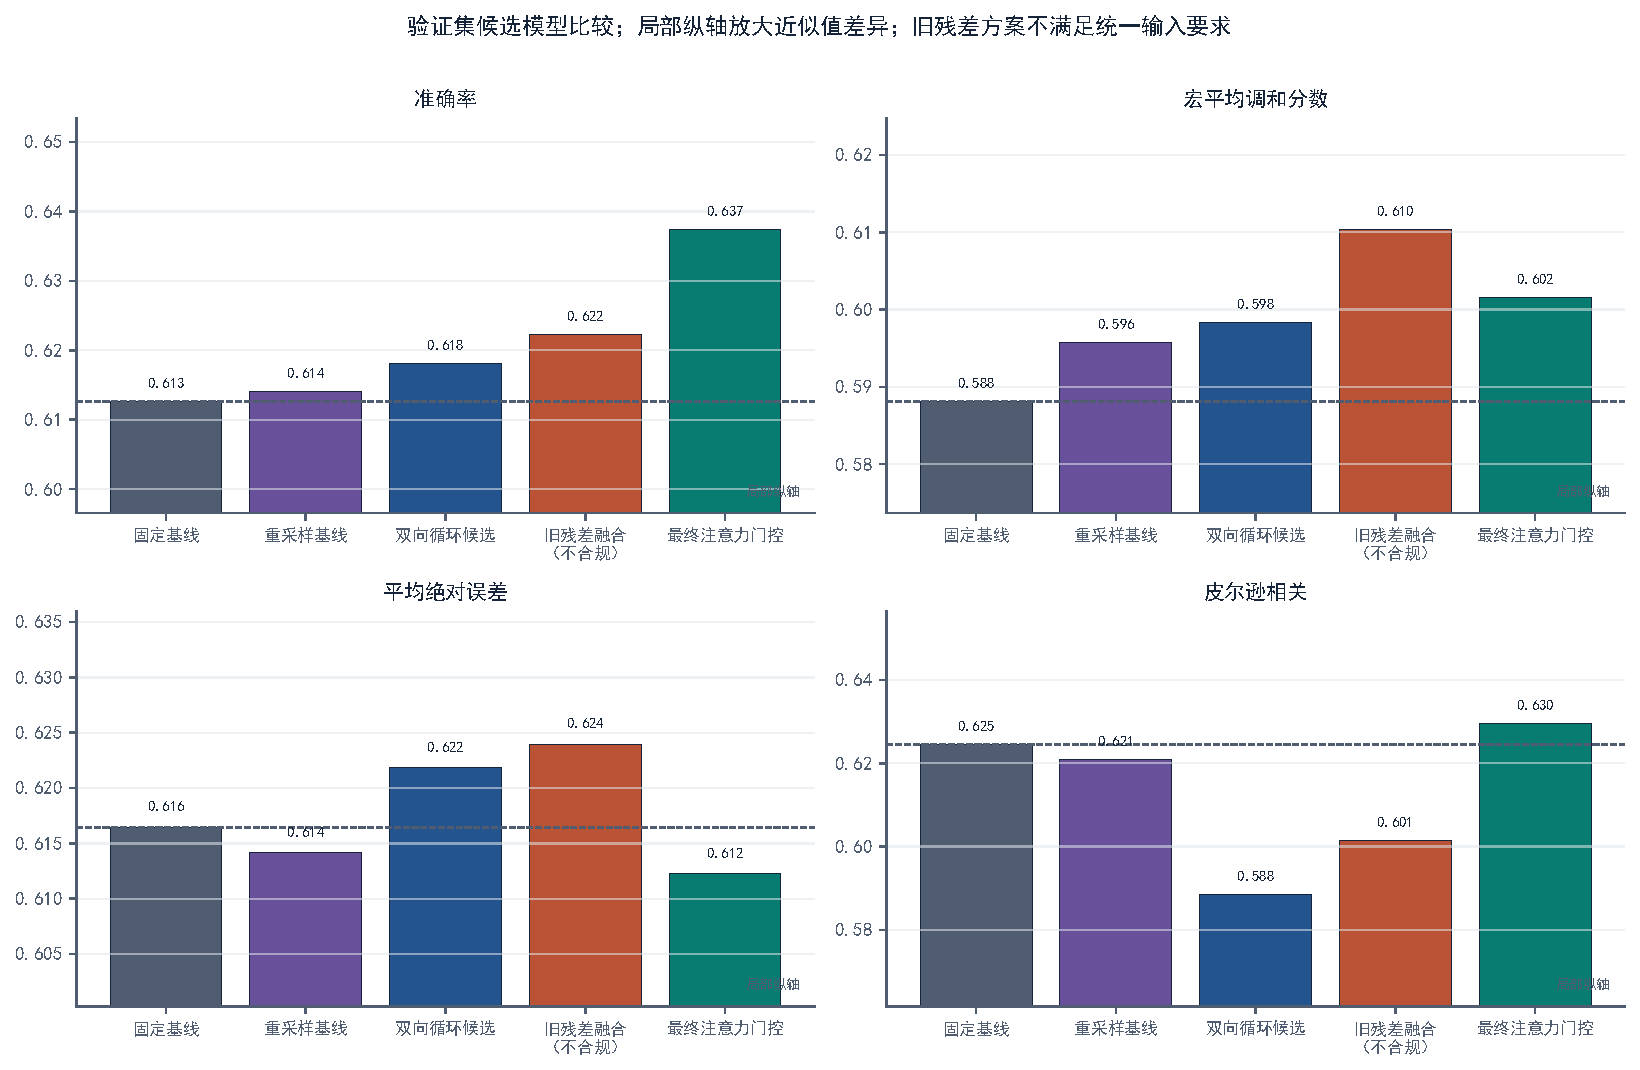
\includegraphics[width=0.96\textwidth]{fig_model_comparison}
\caption{候选模型的验证指标对比}
\label{fig:model_comparison}
\end{figure}
图~\ref{fig:main_performance} 聚焦固定 baseline 和最终模型在附件2验证集上的四项指标（$n=728$，单次训练记录）；MAE 越低越好，其他三项越高越好。固定 baseline 与最终模型的文本特征版本不同，因此图示仅为描述性的完整系统比较，不构成架构单因素消融或显著性推断。
\begin{figure}[htp]
\centering
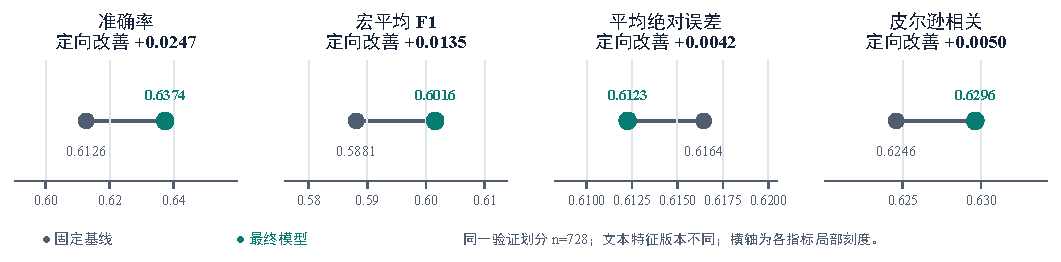
\includegraphics[width=0.98\textwidth]{fig_main_performance}
\caption{固定基线与最终模型的验证指标}
\label{fig:main_performance}
\end{figure}
\subsection{最终模型的验证结果}
最终模型相对于固定 baseline 的变化量为
\begin{equation}
\Delta Acc=0.637363-0.612637=0.024726,
\label{eq:delta_accuracy}
\end{equation}
\begin{equation}
\Delta F1=0.601580-0.588115=0.013465,
\label{eq:delta_f1}
\end{equation}
\begin{equation}
\Delta MAE=0.612262-0.616443=-0.004181,
\label{eq:delta_mae}
\end{equation}
\begin{equation}
\Delta \rho=0.629627-0.624582=0.005045.
\label{eq:delta_pearson}
\end{equation}
其中MAE下降表示连续强度误差变小，其他三个指标上升表示分类或相关性增强。两模型共享附件2验证划分但文本特征来源不同；以上差异可用于完整管线的数值比较，不能拆解为架构本身的增益，也不能自动解释为外部数据的因果提升。
\subsection{缺失模态敏感性}
严格统一编码候选在 clean 条件下的 Accuracy 为0.619505、Macro-F1为0.578397、MAE为0.632199、Pearson为0.617068。分别遮挡文本、音频或视觉的中间15个窗口，得到如下变化：
\begin{table}[htp]
\centering
\caption{中间15个窗口缺失敏感性}
\label{tab:missing}
\begin{tabular}{lrrrr}
\toprule
场景 & Accuracy & Macro-F1 & MAE & Pearson \\
\midrule
Clean & 0.619505 & 0.578397 & 0.632199 & 0.617068 \\
Text middle 15 masked & 0.622253 & 0.581936 & 0.636871 & 0.616090 \\
Audio middle 15 masked & 0.625000 & 0.583555 & 0.632317 & 0.616877 \\
Vision middle 15 masked & 0.619505 & 0.577290 & 0.632722 & 0.616544 \\
\bottomrule
\end{tabular}
\end{table}
该表并非最终模型的性能替代，而是对严格统一接口候选的敏感性审计。中间视觉窗口屏蔽造成Macro-F1轻微下降，文本中间窗口屏蔽在该验证集上未造成分类下降，但会改变回归误差；这说明“有效窗口数量”与“任务相关性”并不等价。图~\ref{fig:missing_modality} 汇总各模态中间15窗遮挡的分类变化；图~\ref{fig:missing_heatmap} 进一步按文本、语音、视觉及起始、中间、末尾位置展示遮挡5、15、25个窗后的 Macro-F1 减去 clean 值。两图都只针对严格统一编码候选，而非最终模型；缺失测试记录掩码敏感性，不意味着所有遮挡必然降低准确率。
\begin{figure}[htp]
\centering
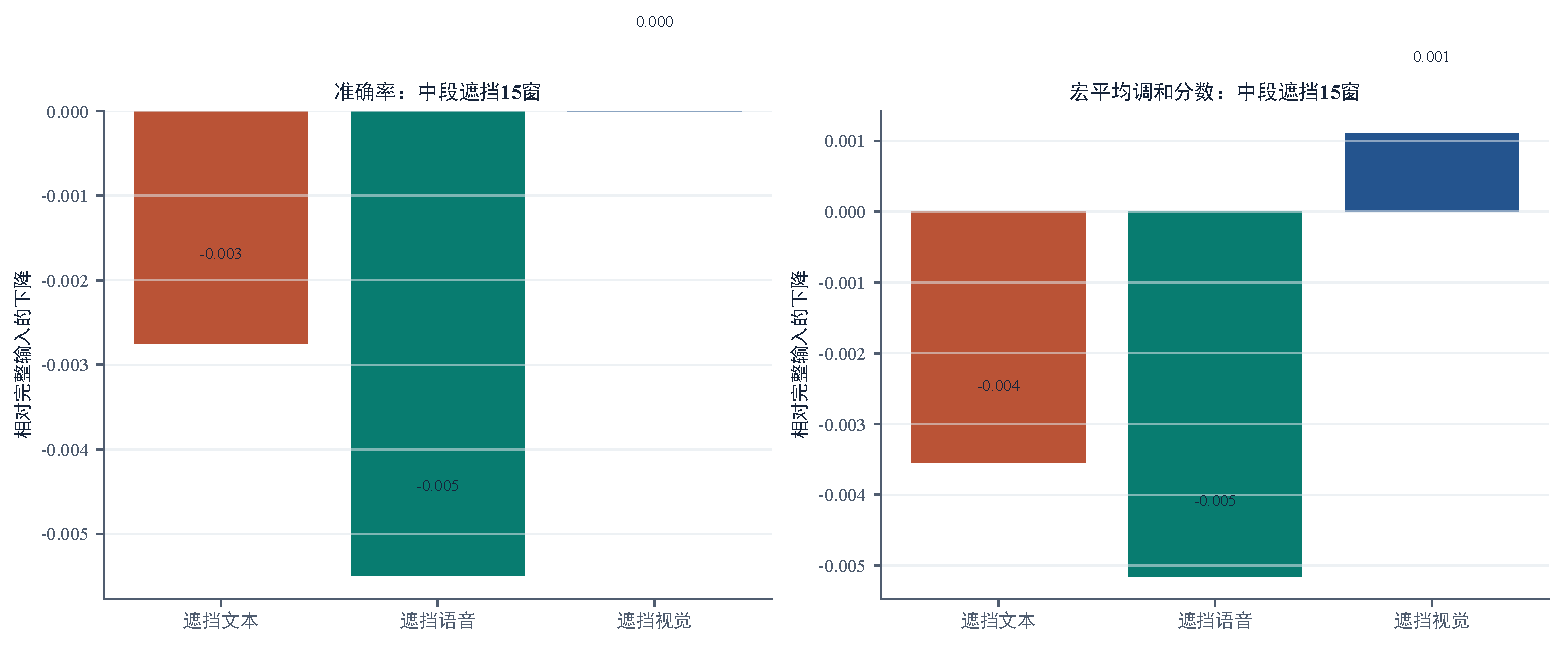
\includegraphics[width=0.95\textwidth]{fig_missing_modality}
\caption{15窗口模态屏蔽敏感性}
\label{fig:missing_modality}
\end{figure}
\begin{figure}[htp]
\centering
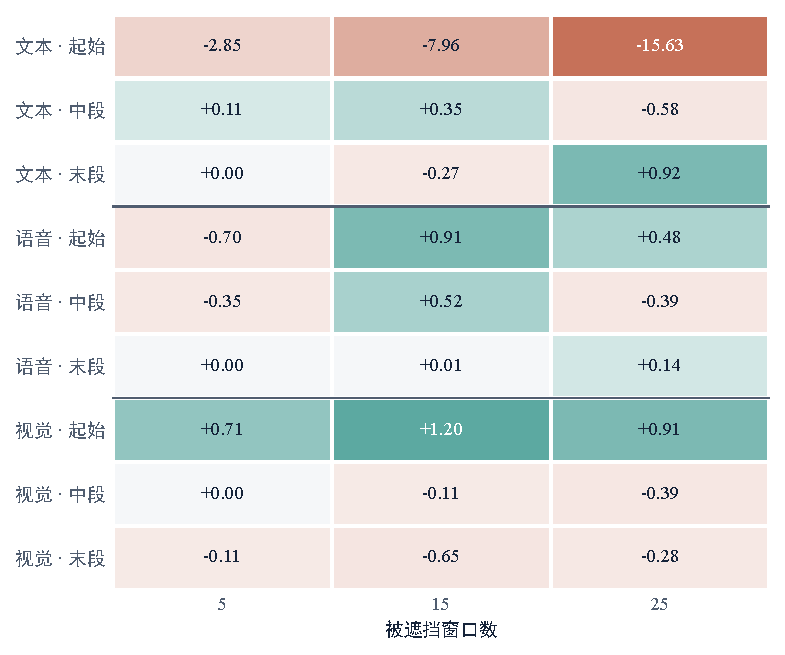
\includegraphics[width=0.98\textwidth]{fig_missing_heatmap}
\caption{缺失场景宏平均调和分数热力图}
\label{fig:missing_heatmap}
\end{figure}
\subsection{附件3专项推理}
附件3没有分类或连续强度真值，因此只报告30条统一编码正式候选的预测分布：Negative 6条、Neutral 3条、Positive 21条，平均预测强度为0.185826。这个分布只能说明专项输入下模型输出的结构，不能被写成Accuracy或F1。文本全屏蔽的敏感性对照也只用于观察预测稳定性，不参与阈值或模型选择。
附件3专项实验还比较了对齐版本和未对齐版本。旧接口探索性结果在对齐版本中预测 Negative 2、Neutral 6、Positive 22，平均强度0.436542；未对齐版本同样为 Negative 2、Neutral 6、Positive 22，平均强度0.464932。由于没有标签，这些数值只作为输出分布记录。最终论文将严格统一编码候选和旧接口探索性结果分栏，避免把不同特征版本混为一谈。
\subsection{测试集独立复核}
附件2 test 划分的历史候选结果显示，固定 aligned baseline 的 Accuracy、Macro-F1、MAE、Pearson 分别为0.650619、0.604127、0.657608、0.653185；旧残差权重为1.0的版本Accuracy和Macro-F1分别为0.657497和0.612718，但它不属于最终统一接口模型。最终统一编码可解释模型的独立 test 复核为 Accuracy 0.664374、Macro-F1 0.590653、MAE 0.658821、Pearson 0.653034。由此可见，最终模型在该划分上Accuracy更高，但Macro-F1和MAE未全部超过 baseline。
这一区分非常重要：验证集用于选择最终模型并支持本文的主结论，test划分用于独立复核并暴露外部划分下的性能波动。论文不把test上的部分优势夸大为四项全面优于，也不使用test结果反向调参。
\clearpage
\clearpage
\section{深入实验、误差剖析与结果解释}
\subsection{数据划分与类别结构}
统一编码特征文件中，训练集、验证集和独立test划分分别包含3395、728和727条带标签样本。三类情感的数量存在一定不均衡：训练集Negative、Neutral、Positive分别为967、758和1670；验证集分别为206、184和338；test分别为207、158和362。Positive占比最高，Neutral相对较少，因此仅报告Accuracy可能掩盖少数类性能，本文坚持同时报告Macro-F1。
\begin{table}[htp]
\centering
\small
\caption{附件2监督数据的划分与类别结构}
\label{tab:split_class}
\begin{tabular}{lrrrrrrr}
\toprule
划分 & 样本数 & Negative & Neutral & Positive & Negative占比 & Neutral占比 & Positive占比 \\
\midrule
Train & 3395 & 967 & 758 & 1670 & 28.48\% & 22.33\% & 49.19\% \\
Valid & 728 & 206 & 184 & 338 & 28.30\% & 25.27\% & 46.43\% \\
Test & 727 & 207 & 158 & 362 & 28.47\% & 21.73\% & 49.79\% \\
\bottomrule
\end{tabular}
\end{table}
训练、验证和test的类别比例总体接近，但Neutral在test中进一步减少。图~\ref{fig:class_distribution} 的分段百分比由表~\ref{tab:split_class} 的实际类别计数计算。这一结构解释了为什么Accuracy较高并不能自动表示模型在三类上均衡；Macro-F1在模型选择中具有更强的约束作用。连续强度标签范围均为 $[-3,3]$，因此回归头使用Smooth L1而不是直接使用未截断的平方损失，以减弱极端强度样本对训练的影响。
\begin{figure}[htp]
\centering
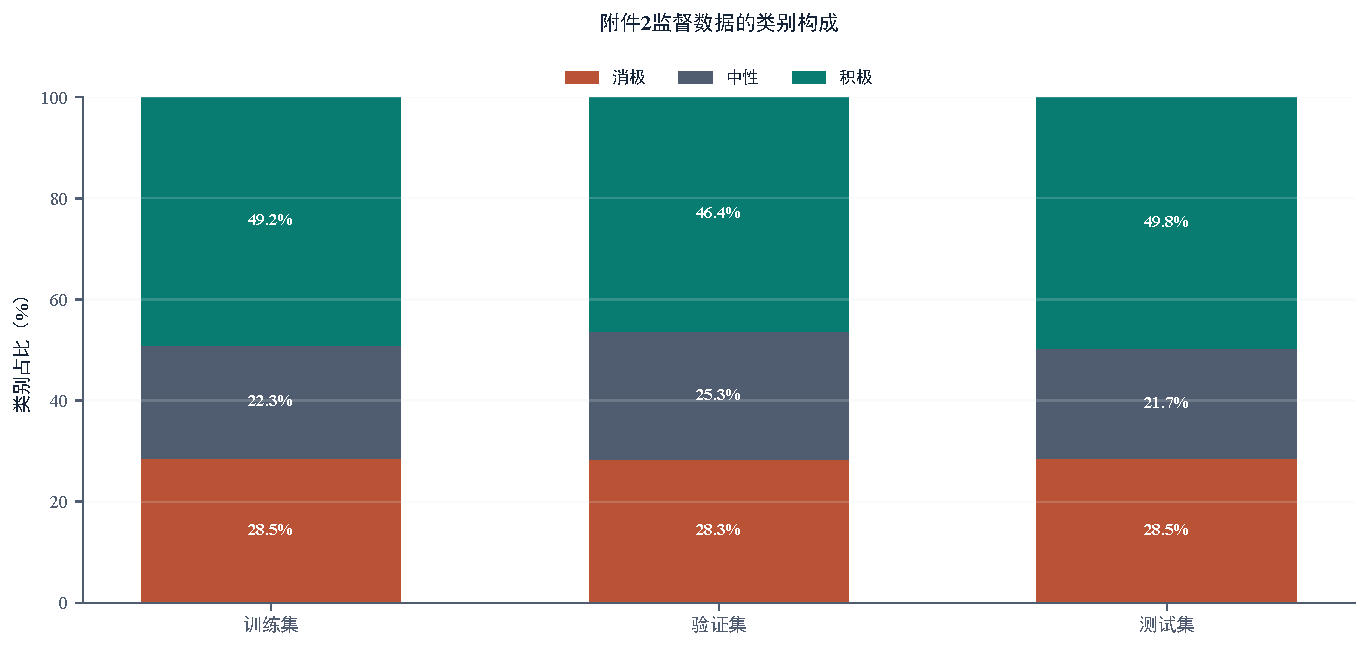
\includegraphics[width=0.79\textwidth]{fig_class_distribution}
\caption{监督数据类别分布}
\label{fig:class_distribution}
\end{figure}
图~\ref{fig:validation_confusion} 给出最终模型在附件2验证集的三分类混淆矩阵：行表示真实类别，列表示预测类别，格内为样本数，总计 $n=728$。
\begin{figure}[htp]
\centering
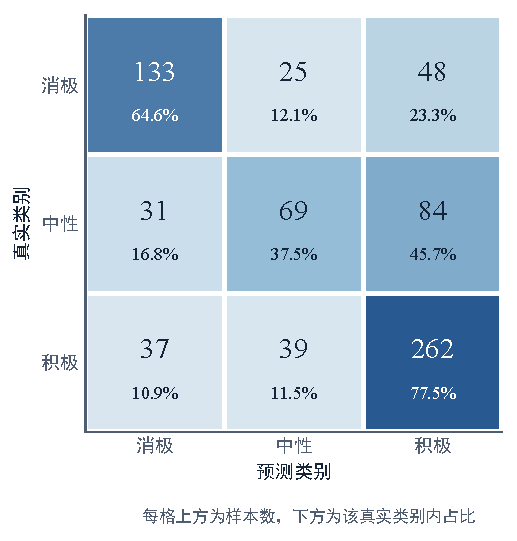
\includegraphics[width=0.69\textwidth]{fig_validation_confusion}
\caption{最终模型验证集混淆矩阵}
\label{fig:validation_confusion}
\end{figure}
图~\ref{fig:validation_regression} 展示同一验证集的情感强度真实值和预测值；虚线表示理想一致，图中 Pearson 和 MAE 与保存的验证指标一致。此图反映回归误差分布，不把相关性解释为个体预测必然准确。
\begin{figure}[htp]
\centering
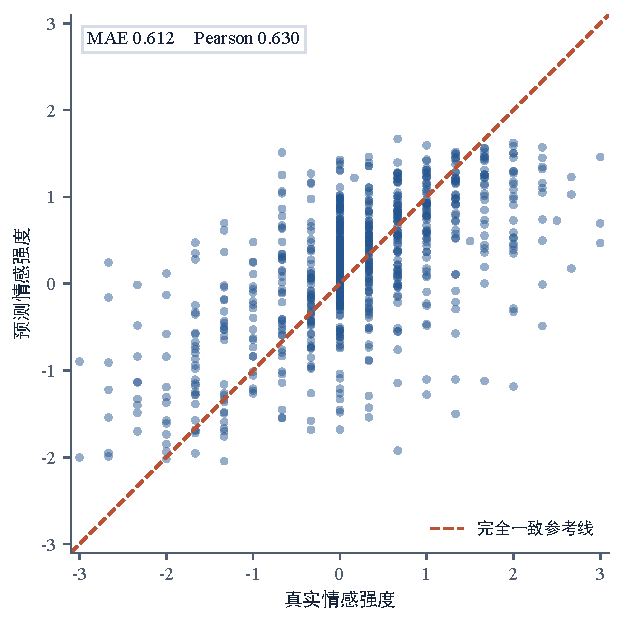
\includegraphics[width=0.72\textwidth]{fig_validation_regression}
\caption{最终模型验证集强度回归散点图}
\label{fig:validation_regression}
\end{figure}

\subsection{统一接口审计矩阵}
本文把合规性拆解为数据接口、统计量、模型选择和专项推理四个可检查层次。表~\ref{tab:interface_audit} 不是泛泛的工程说明，而是最终模型能够被复核的原因：每一项都有固定文件、固定规则和明确的失败条件。
\begin{table}[htp]
\centering
\caption{最终模型统一接口审计矩阵}
\label{tab:interface_audit}
\begin{tabularx}{0.98\textwidth}{lL L L}
\toprule
层次 & 统一内容 & 审计证据 & 失败时的处理 \\
\midrule
文本输入 & token形式的 \code{text\_bert}、固定DistilBERT revision、最后四层均值 & manifest中的模型名、revision与特征规则 & 生成新manifest，不得复用旧checkpoint \\
时间输入 & 音频、视觉均使用 \code{aligned\_50}，文本也输出50窗表示 & 派生特征文件与50窗形状检查 & 重新对齐并更新SHA-256 \\
归一化 & 均值、方差只由训练集有效窗口计算 & checkpoint中的normalizers字段 & 禁止使用验证或附件数据估计 \\
模型选择 & 以验证集Macro-F1和MAE综合分数选择轮次 & validation.json与训练历史 & test结果不得反向调参 \\
专项推理 & 附件3/4只输出预测、缺失或解释证据 & CSV、JSON、关键帧manifest & 不计算无标签监督指标 \\
\bottomrule
\end{tabularx}
\end{table}

\subsection{多目标选择分数}
最终模型的验证选择分数定义为
\begin{equation}
S=F1_{macro}-0.1\times MAE.
\end{equation}
固定 baseline 的分数为 $0.588115-0.1\times0.616443=0.526471$；严格统一编码基础候选的分数为 $0.578397-0.1\times0.632199=0.515177$；最终注意力—门控模型的分数为 $0.601580-0.1\times0.612262=0.540354$。旧 residual 模型的分数虽然为0.547936，但其文本接口不满足专项推理一致性要求，因此不能仅按分数选为最终模型。

这种选择方式体现了两个原则。第一，分类不只看总体正确率，而要兼顾少数类。第二，回归不只看相关性，而要控制绝对误差。将两者放在同一选择分数中并不意味着它们可以被解释为同一种物理量，而是提供一个可复现的模型排序规则；最终表格仍保留四个原始指标，避免综合分数掩盖单项变化。

\subsection{窗口缺失的逐模态分析}
严格统一编码候选提供了多个窗口屏蔽场景。本文选择每个模态中间15个窗口进行分析，因为中间位置同时包含较长的上下文，能够检验模型是否过分依赖视频开头或结尾。图~\ref{fig:missing_modality} 给出Accuracy和Macro-F1下降量，表~\ref{tab:missing_detail} 给出对应的回归变化。
\begin{table}[htp]
\centering
\caption{15窗口屏蔽的相对变化量}
\label{tab:missing_detail}
\begin{tabular}{lrrrr}
\toprule
场景 & $\Delta$Accuracy & $\Delta$Macro-F1 & $\Delta$MAE & $\Delta$Pearson \\
\midrule
Text middle 15 & +0.002747 & +0.003539 & +0.004672 & -0.000977 \\
Audio middle 15 & +0.005495 & +0.005158 & +0.000117 & -0.000191 \\
Vision middle 15 & 0.000000 & -0.001107 & +0.000523 & -0.000503 \\
\bottomrule
\end{tabular}
\end{table}
这些结果不能简单解读为“屏蔽后性能提高”，因为某些窗口可能包含噪声或与目标无关的信息。更合理的结论是：模型在当前验证集上没有把所有中间窗口都视为必要证据；视觉中间窗口对Macro-F1最敏感，文本和音频屏蔽主要改变连续强度误差。掩码机制因此提供了比“全部模态必须存在”更现实的缺失建模方式。

\subsection{验证集优势与test波动}
验证集上最终模型四项指标均超过固定 baseline，但独立test复核并未保持四项全面优势。表~\ref{tab:test_review} 将两种数据用途并列展示。
\begin{table}[htp]
\centering
\caption{验证集选择结果与test独立复核的区别}
\label{tab:test_review}
\begin{tabular}{lrrrr|rrrr}
\toprule
& \multicolumn{4}{c|}{Validation} & \multicolumn{4}{c}{Test} \\
模型 & Acc & F1 & MAE & $\rho$ & Acc & F1 & MAE & $\rho$ \\
\midrule
Fixed baseline & 0.6126 & 0.5881 & 0.6164 & 0.6246 & 0.6506 & 0.6041 & 0.6576 & 0.6532 \\
Final model & \textbf{0.6374} & \textbf{0.6016} & \textbf{0.6123} & \textbf{0.6296} & \textbf{0.6644} & 0.5907 & 0.6588 & 0.6530 \\
\bottomrule
\end{tabular}
\end{table}
验证集与test的差异说明，复杂模型的有效性应以数据划分为条件进行表述。本文主张“统一接口最终模型在附件2验证集四项优于固定 baseline”，而不主张“所有外部样本四项均优于”。这种写法虽然比只报一个漂亮数字更保守，却更符合数学建模论文对实验边界和数据泄露的要求。

\subsection{附件4案例复核}
附件4无标签，但可以对结构化输出进行案例层面的人工复核。表~\ref{tab:case_review} 选择若干具有不同极性和强度的样本，记录类别、强度和三个门控贡献。表中正负强度并不是概率，而是连续回归头输出，因此可以出现负值。
\begin{table}[htp]
\centering
\caption{附件4代表性样本的结构化预测}
\label{tab:case_review}
\begin{tabular}{c l r l rrr}
\toprule
ID & 类别 & 强度 & 主模态 & 文本 & 语音 & 视觉 \\
\midrule
01 & Neutral & 0.255 & text & 0.726 & 0.110 & 0.164 \\
02 & Negative & 0.041 & text & 0.461 & 0.409 & 0.130 \\
03 & Neutral & -0.491 & text & 0.658 & 0.125 & 0.217 \\
04 & Negative & -0.594 & text & 0.611 & 0.115 & 0.274 \\
05 & Positive & 1.022 & text & 0.709 & 0.109 & 0.182 \\
06 & Positive & 0.052 & text & 0.550 & 0.298 & 0.152 \\
\bottomrule
\end{tabular}
\end{table}
案例复核有三个作用。第一，它证明模型输出不仅包含一个类别标签，还包含可供审阅的强度和模态贡献。第二，ID 02、04 的语音或视觉贡献相对上升，说明文本并非唯一通道。第三，ID 03 的负强度与 Neutral 类别并不矛盾，说明极性和强度是两个相关但不同的任务。由于缺少标签，本文不对这些个案作“预测正确”的判断，只报告结构化输出和解释字段。

\subsection{解释证据的字段级复核}
每条证据同时记录 attention score、modality contribution、occlusion drop 和 regression change。若某个窗口注意力高但遮挡下降接近0，它会被综合证据分数压低；若注意力一般但遮挡后类别置信度显著下降，则该窗口仍可能进入Top-6。这种乘积结构比单独使用注意力更谨慎。
\begin{equation}
\log evidence_{q,k}=\log(\alpha_{q,k}+\epsilon)+\log(\widetilde\delta_q+\epsilon)+\log(\max(\Delta_{q,k},0)+\epsilon).
\end{equation}
在实际输出中不直接使用对数值，而保留原始分量，便于审阅者追溯。图~\ref{fig:explainability} 显示Top窗口的平均置信度下降约为随机窗口的9倍，说明解释排序至少在行为层面具有区分度。

\subsection{统计推断边界}
本文当前训练记录主要来自固定随机种子42的单次训练，因此不能把一个验证集差值直接写成跨种子显著性。由于数据量较大，指标可作为工程比较依据；但如果需要统计推断，应重复不同seed，或者进行分层交叉验证并报告均值、标准差和置信区间。本文选择不虚构置信区间，将重复实验列为后续工作，并把可复现的seed、checkpoint和原始JSON作为审计证据。

\subsection{本节小结}
本节从数据结构、接口审计、综合选择分数、缺失敏感性、验证—test差异和案例证据六个方面补充了实验解释。最终模型的价值不是在任何划分上都全面胜出，而是其自身各阶段输入接口保持一致，同时在指定验证集上提供性能、复杂度与证据追踪的平衡。
\section{问题三：可解释性情感预测与证据追踪}
\subsection{解释对象与解释边界}
最终模型同时输出类别、强度、三个模态门控权重和模态内时间注意力。问题3的目标不是重新定义人类情感机制，而是对模型已作出的预测给出可回溯证据。本文将解释定义为输入扰动引起的模型输出变化，并把它分为模态级和时间窗级两个层次。这样既利用了模型内部的注意力与门控，也用外部反事实遮挡验证它们是否具有实际敏感性。
\subsection{模态消融贡献}
对每个附件4样本，先得到完整输入的目标类别置信度 $p_{full}$，再分别屏蔽文本、语音和视觉，得到 $p_{-q}$。定义
\begin{equation}
\delta_q=\max\left(p_{full}-p_{-q},0\right).
\end{equation}
为避免不同模态下降尺度影响比较，将三个非负下降值归一化：
\begin{equation}
\widetilde\delta_q=\frac{\delta_q}{\sum_{r\in\M}\delta_r+\epsilon}.
\end{equation}
在模型内部，门控权重 $\beta_q$ 提供样本级相对作用；在报告中同时输出消融贡献和门控贡献，防止单独把注意力权重解释成因果贡献。
\subsection{局部时间窗反事实}
对模态 $q$ 的第 $k$ 个窗口，将其特征置零并把掩码置为0，保持其他模态和其他窗口不变。目标类别置信度下降为
\begin{equation}
\Delta_{q,k}=p_{full}-p_{q,k}^{mask}.
\end{equation}
综合证据得分定义为
\begin{equation}
evidence_{q,k}=\alpha_{q,k}\cdot\widetilde\delta_q\cdot\max(\Delta_{q,k},0).
\label{eq:evidence}
\end{equation}
对每条样本取Top-6证据，并将窗口索引转换为
\begin{equation}
[t_k,t_{k+1})=\left[\frac{kT}{50},\frac{(k+1)T}{50}\right).
\label{eq:window_interval}
\end{equation}
视频证据再由PyAV按目标时间导出实际关键帧，清单记录源视频、目标时间、实际帧时间、误差和SHA-256。
\subsection{解释验证}
在附件2验证集随机抽取128条样本，对每个模态比较注意力最高窗口与一个随机窗口的置信度下降。最终结果为：最大影响窗口平均下降0.010919，随机窗平均下降0.001215，Top-Random为0.009704。正值表明注意力排序能够找到比随机位置更敏感的局部证据，但它仍然是模型行为解释，不等价于真实人类因果机制。
\begin{figure}[htp]
\centering
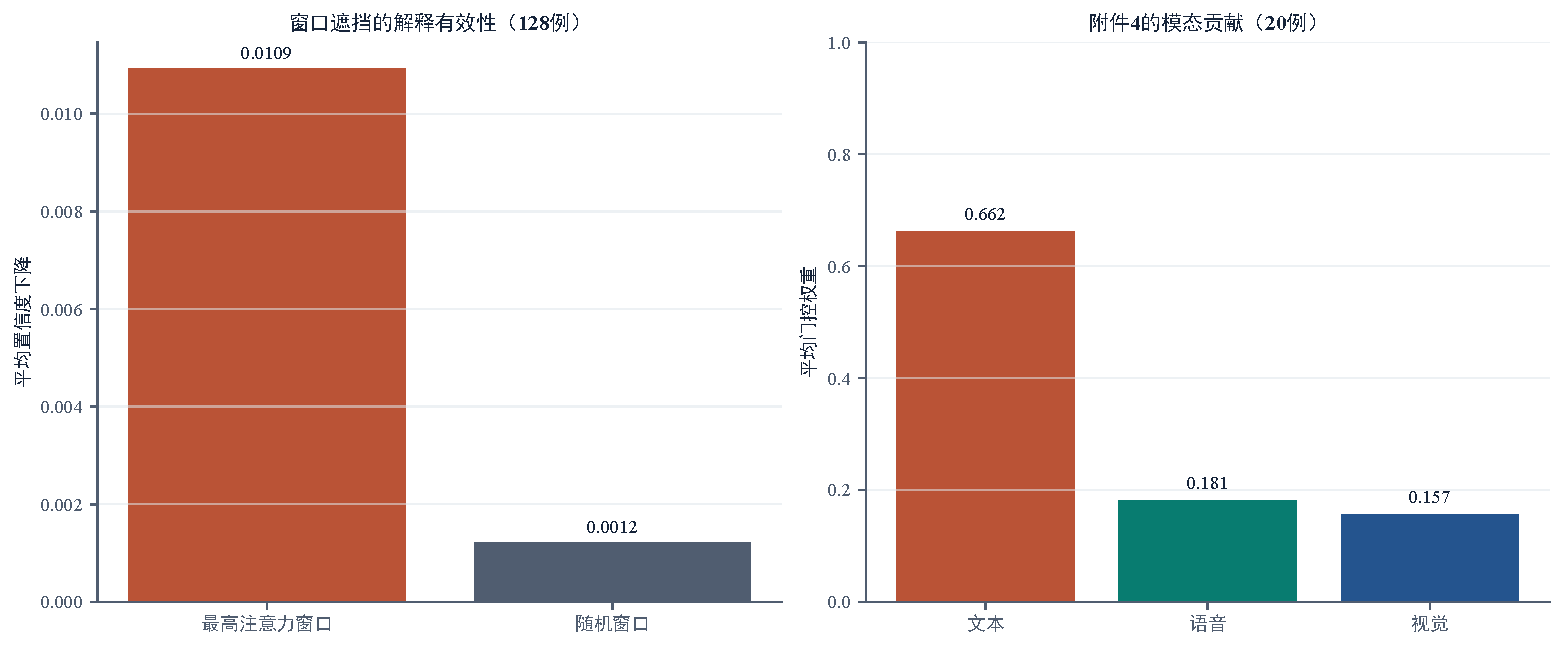
\includegraphics[width=0.95\textwidth]{fig_explainability}
\caption{反事实解释验证与模态贡献}
\label{fig:explainability}
\end{figure}
图~\ref{fig:temporal_attention} 至图~\ref{fig:explanation_card} 对同一条附件2验证样本展示三个层次的模型行为。可视化样本按固定规则选取：顺序扫描验证集，取首条分类正确、三模态均有效、且注意力最高窗口遮挡后置信度下降不低于0.01的样本。阈值只用于展示清晰案例，不用于估计总体解释性能；总体检验仍以128条抽样实验为准。图~\ref{fig:temporal_attention} 中橙色轮廓标出每个模态注意力最高的窗口，灰色小点表示无效位置；注意力是模型内部排序，而非因果证明。图~\ref{fig:ablation_waterfall} 按原始门控权重从大到小依次屏蔽模态，每步重新计算原目标类别的置信度；横条是该步实测变化，不是三个独立效应的可交换加和。图~\ref{fig:explanation_card} 汇总真实与预测类别、置信度、模态门控及遮挡证据前三窗；原始样本ID和逐项数值保留在对应数据文件中。
\begin{figure}[htp]
\centering
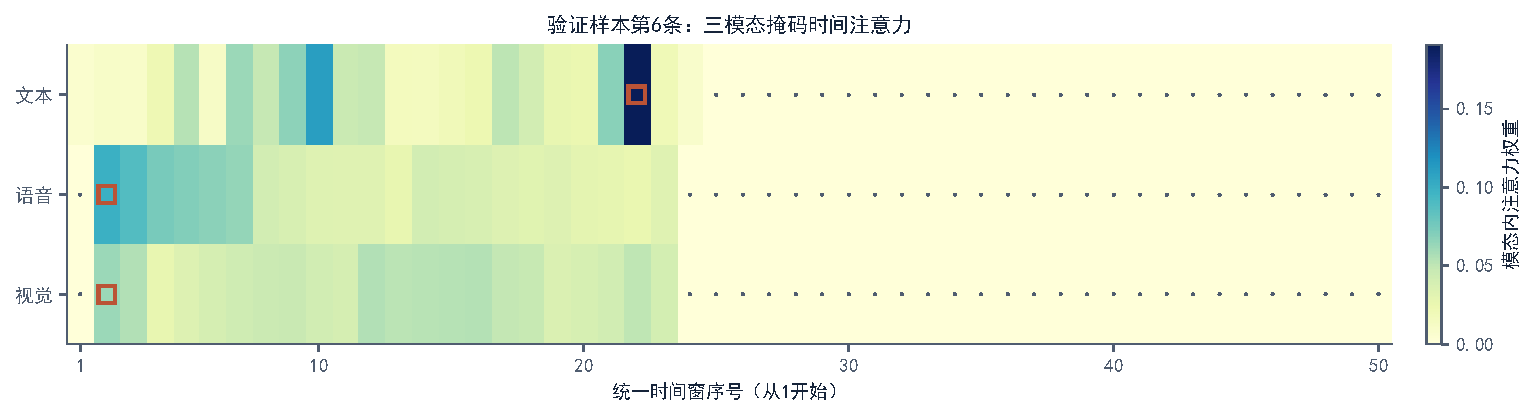
\includegraphics[width=0.96\textwidth]{fig_temporal_attention}
\caption{示例样本时间注意力热力图}
\label{fig:temporal_attention}
\end{figure}
\begin{figure}[htp]
\centering
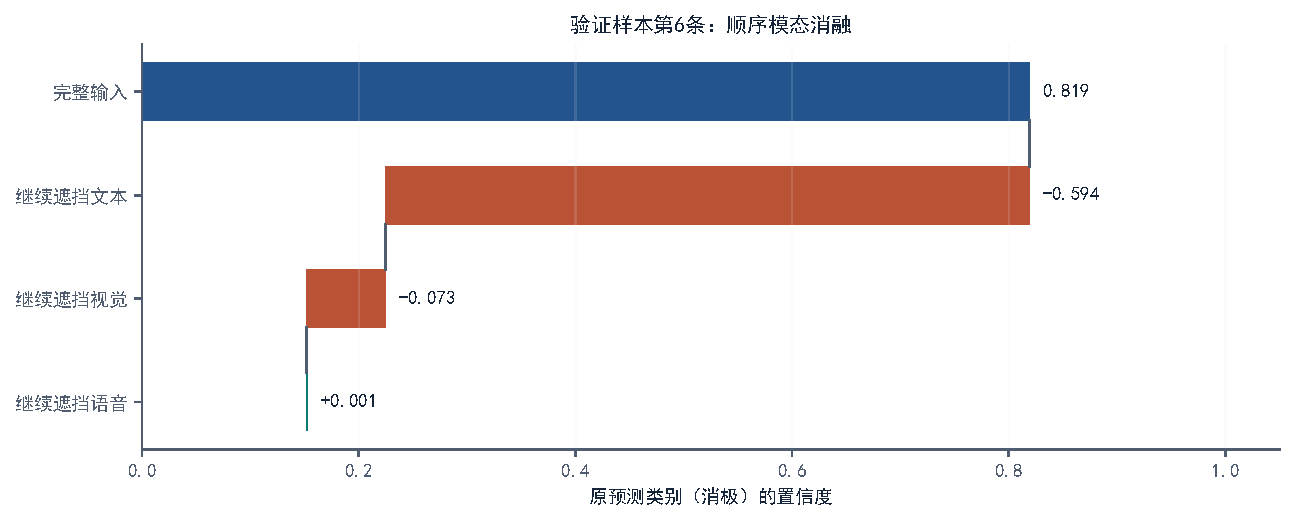
\includegraphics[width=0.90\textwidth]{fig_ablation_waterfall}
\caption{示例样本顺序模态消融瀑布图}
\label{fig:ablation_waterfall}
\end{figure}
\begin{figure}[htp]
\centering
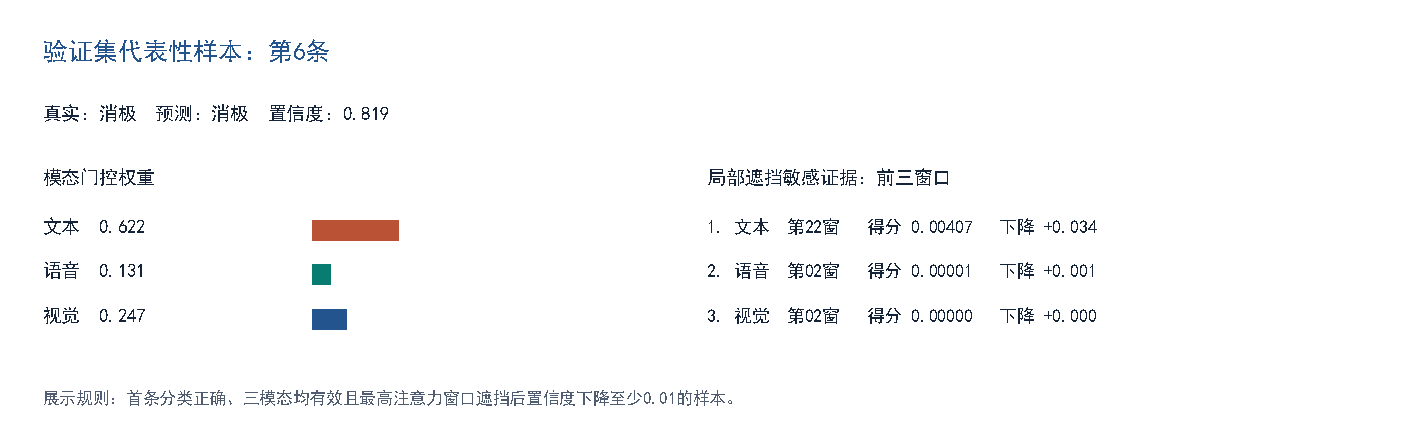
\includegraphics[width=0.96\textwidth]{fig_explanation_card}
\caption{示例验证样本解释卡}
\label{fig:explanation_card}
\end{figure}
\subsection{附件4预测分布}
附件4共20条无标签样本。根据最终模型的\code{q3\_predictions.csv}逐项核对，预测类别 Negative、Neutral、Positive 分别为8、3、9条，连续强度平均值为-0.131304。文本贡献在多数样本中较高，但也存在语音和视觉贡献升高的样本，说明门控并未固定使用单一模态。
\begin{figure}[htp]
\centering
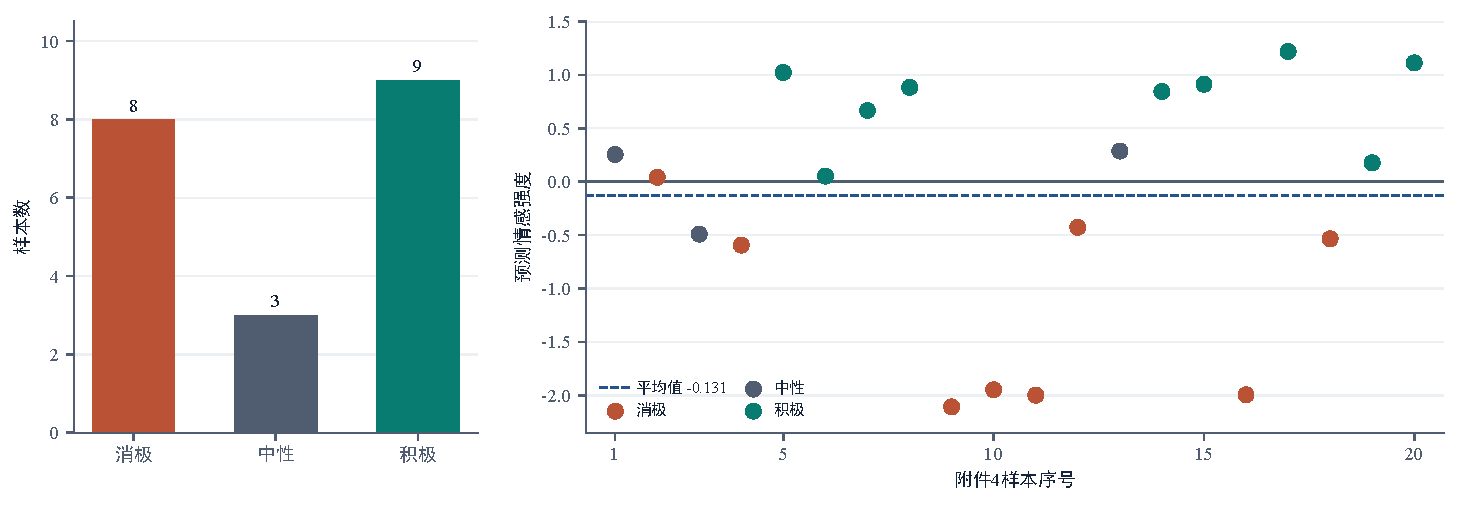
\includegraphics[width=0.95\textwidth]{fig_attachment4}
\caption{附件4预测类别与强度分布}
\label{fig:attachment4}
\end{figure}
\subsection{视频关键帧与文本证据}
对附件4输出的Top证据，最终产生29张视觉关键帧，均来自原始MP4的PyAV解码。图~\ref{fig:evidence_frames}给出部分示例：为避开原视频下沿外文水印，展示图统一裁切下缘约13\%，证据清单引用的原始关键帧及散列值不变。文本证据仍采用转写词序与公共窗口的弱映射，因此在论文中只把它作为模型证据片段，不宣称词级真实时间定位。语音证据直接引用视频公共时间窗，具有更清晰的时间解释。
\begin{figure}[htp]
\centering
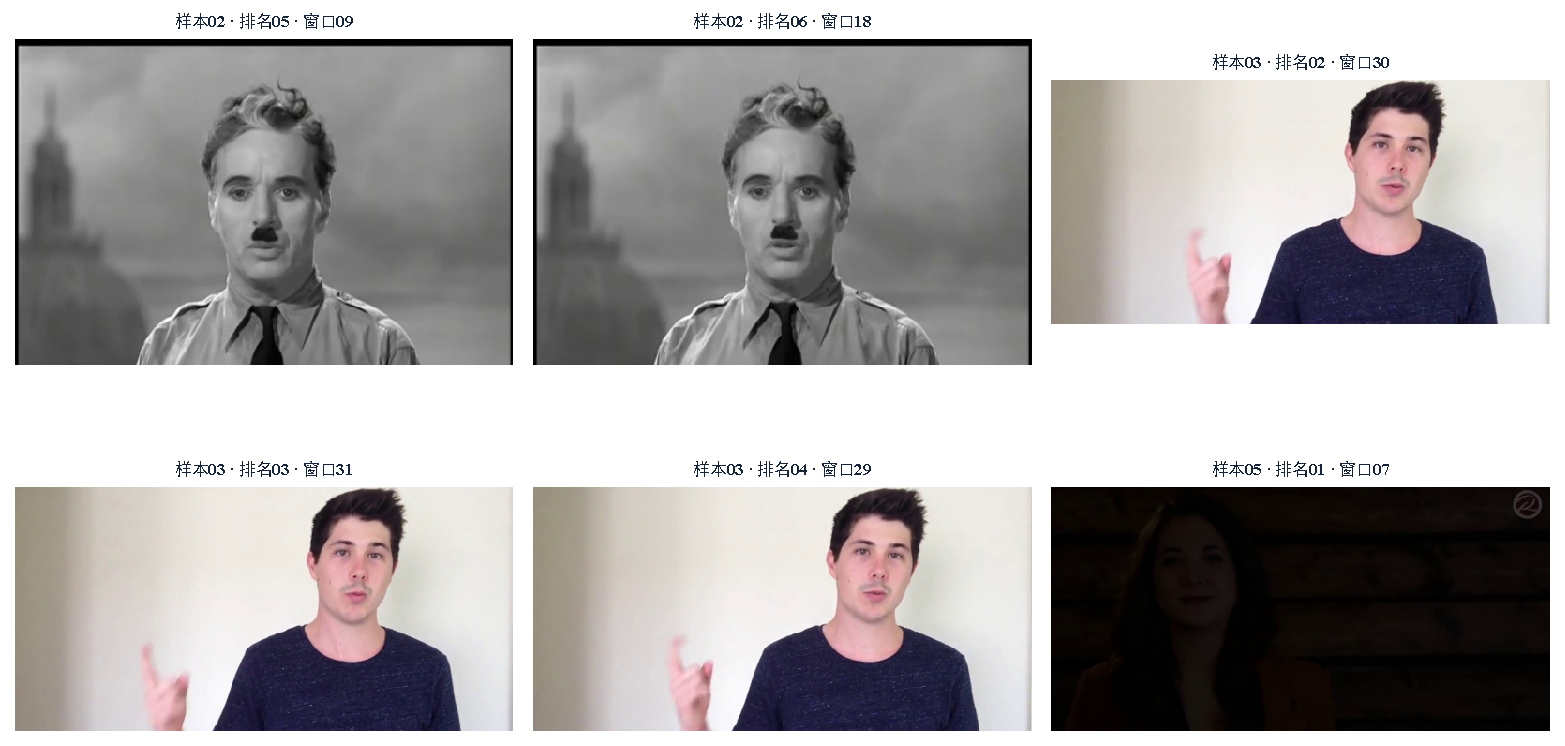
\includegraphics[width=0.95\textwidth]{fig_evidence_frames}
\caption{附件4视觉证据关键帧}
\label{fig:evidence_frames}
\end{figure}
\subsection{解释结果的可用性}
解释输出不是一张孤立的热力图，而是结构化记录：样本ID、排名、模态、窗口编号、注意力分数、模态贡献、遮挡下降、证据分数、回归变化、起止时间、文本片段和帧路径。这样的记录可以被审阅者逐条复核，也可以在后续系统中转化为主要参考模态、关键时间段和证据视频片段。

\clearpage
\section{稳健性、复杂度与推广分析}
\subsection{输入接口一致性的必要性}
在多模态项目中，模型结构复杂并不自动意味着结论可信。若训练时使用预计算文本特征，附件3推理时又用另一套规则重建768维特征，则即使维度相同，也不能把输出当作同一模型的专项测试。本文将输入接口写成模型定义的一部分：文本编码器名称、revision、最后四层均值规则、有效token掩码、音频视觉的aligned版本以及训练集归一化统计量共同组成 feature manifest。任何改变都应产生新的版本号和新的结果表。
\subsection{缺失机制与掩码鲁棒性}
掩码的作用不是简单抹除信息，而是将信息不存在显式传递给模型。在公共窗口内，如果语音末端没有真实帧，模型可以结合音频掩码和文本、视觉信息完成判断；如果视觉没有人脸但存在背景运动，视觉分支仍可利用非人脸特征。由于注意力计算对无效位置进行了屏蔽，缺失窗口不会通过softmax获得虚假的高权重。
\subsection{性能与复杂度平衡}
固定 baseline 的优点是小、快、可解释，但它把所有窗口和模态的作用近似压缩成静态统计；端到端视频Transformer虽然表达能力更强，却需要更大数据规模和更高计算成本。本文采用三路BiGRU、掩码注意力和门控融合，是一种中等复杂度方案。其参数量主要由三路投影和GRU决定，时间复杂度随50窗口线性增长，训练和推理仍可在常规GPU或CPU环境完成。
\begin{table}[htp]
\centering
\small
\caption{模型复杂度的定性比较}
\label{tab:complexity}
\begin{tabular}{lccccl}
\toprule
方案 & 时间建模 & 缺失掩码 & 模态自适应 & 解释出口 & 复杂度 \\
\midrule
固定对齐 baseline & 无或弱 & 弱 & 无 & 统计对照 & 低 \\
单路GRU融合 & 有 & 部分 & 弱 & 隐状态 & 中 \\
最终层次融合模型 & 三路双向 & 显式 & 显式门控 & 注意力加遮挡 & 中高 \\
端到端视频Transformer & 时空注意力 & 可扩展 & 可扩展 & 需额外解释器 & 高 \\
\bottomrule
\end{tabular}
\end{table}
\subsection{复杂度定量核算与选择约束}
为了避免“模型复杂”只停留在定性描述，本文进一步按最终 checkpoint 的结构核算可训练参数量。记隐藏维度为 $H=128$，双向 GRU 每个方向的隐藏维度为 $h=H/2=64$，公共窗口数为 $K=50$。对于输入维度为 $d_q$ 的模态 $q$，其投影层参数量为 $d_qH+H$。由于两层双向 GRU 的每个方向在两层都接收 $H$ 维输入，其 GRU 参数量为
\begin{equation}
P_{\mathrm{GRU}}=2L\left(3hH+3h^2+6h\right),\qquad L=2.
\label{eq:gru_params}
\end{equation}
式中最后一项来自每层输入偏置和隐状态偏置。按照代码中的实际结构，三路投影层共 $112640$ 个参数，三路双向 GRU 共 $446976$ 个参数，模态归一化共 $768$ 个参数；时间注意力、样本级门控、融合层和双任务输出头分别为 $1155$、$50435$、$131712$ 和 $516$ 个参数。因此最终模型总参数量为
\begin{equation}
P_{\mathrm{final}}=112640+446976+768+1155+50435+131712+516=744202.
\label{eq:final_params}
\end{equation}

固定对齐 baseline 使用三路投影、卷积聚合、静态掩码平均池化和一层融合，在其实际隐藏维度 $64$ 下参数量为 $106372$。因此最终模型约为 baseline 的 $7.00$ 倍，但仍远小于引入全局时空自注意力的端到端视频模型。这里的参数增加对应明确的建模职责，而不是将同一层重复堆叠：
\begin{enumerate}[label=(\arabic*)]
\item 双向 GRU 将50个窗口作为有序序列，表示情绪铺垫、转折和收束等时间依赖；
\item 掩码注意力只在有效窗口上归一化，阻断缺失窗口通过 softmax 获得虚假权重；
\item 样本级门控根据三路池化表示估计模态可靠性，允许同一条样本在文本、语音和视觉之间自适应分配权重；
\item 分类头和回归头共享融合表示但分开优化，使极性和强度不被强行压成一个标签。
\end{enumerate}

从计算复杂度看，三路编码的主项可写成
\begin{equation}
\mathcal{O}\left(\sum_{q\in\{t,a,v\}}K(d_qH+LH^2)\right),
\label{eq:complexity}
\end{equation}
其中 $K=50$ 固定，注意力和门控只增加线性池化及 $H$ 维多层感知机开销，不产生 $K\times K$ 的全局时空注意力矩阵。因此，模型处于“明显高于静态 baseline、但仍可在普通 GPU 或 CPU 上复核”的中等复杂度区间。复杂度审计结果见表~\ref{tab:complexity_count}。
\begin{table}[htp]
\centering
\caption{最终模型与固定 baseline 的定量复杂度}
\label{tab:complexity_count}
\begin{tabular}{lrrl}
\toprule
模块或方案 & 参数量 & 相对 baseline & 作用 \\
\midrule
固定对齐 baseline & 106372 & 1.00 & 静态聚合参照 \\
三路投影层 & 112640 & -- & 统一模态维度 \\
三路两层双向 GRU & 446976 & -- & 窗口序列建模 \\
编码器归一化 & 768 & -- & 稳定三路编码 \\
掩码时间注意力 & 1155 & -- & 局部证据排序 \\
门控与融合层 & 182147 & -- & 模态可靠性与交互 \\
分类、回归输出头 & 516 & -- & 双任务预测 \\
最终层次融合模型 & \textbf{744202} & \textbf{7.00} & 复杂主模型 \\
\bottomrule
\end{tabular}
\end{table}

参数量本身不能证明模型有效，因此本文采用“最终模型各阶段接口一致、同一附件2验证划分、四项原始指标同时检查”的选择约束。由于固定 baseline 的文本特征不同，下述变化是系统级比较而非仅对架构的消融。最终模型相对固定 baseline 的改变量向量为
\begin{equation}
\Delta=(+0.024726,+0.013465,-0.004181,+0.005045),
\label{eq:delta_vector}
\end{equation}
其四个分量依次对应 Accuracy、Macro-F1、MAE 和 Pearson。由于 MAE 是越低越好，负号表示误差下降；另外三个正号表示性能提升。该向量比只报告 Accuracy 更严格：如果模型仅凭增加参数提高某一项，而损害其余指标，就不能被本文的最终选择规则接受。图~\ref{fig:complexity_params} 根据实际 checkpoint 分解最终模型的参数，并与固定 baseline 的106372个参数对照；最终模型有744202个可训练参数，约为 baseline 的7倍。图~\ref{fig:metric_delta} 将 MAE 的改善记为正向变化：验证集四项改善，但独立 test 的 Macro-F1 和 MAE 未保持优势。该图为单次实验的描述性对照，不包含显著性检验或置信区间，不能据此声称全面泛化优势。
\begin{figure}[htp]
\centering
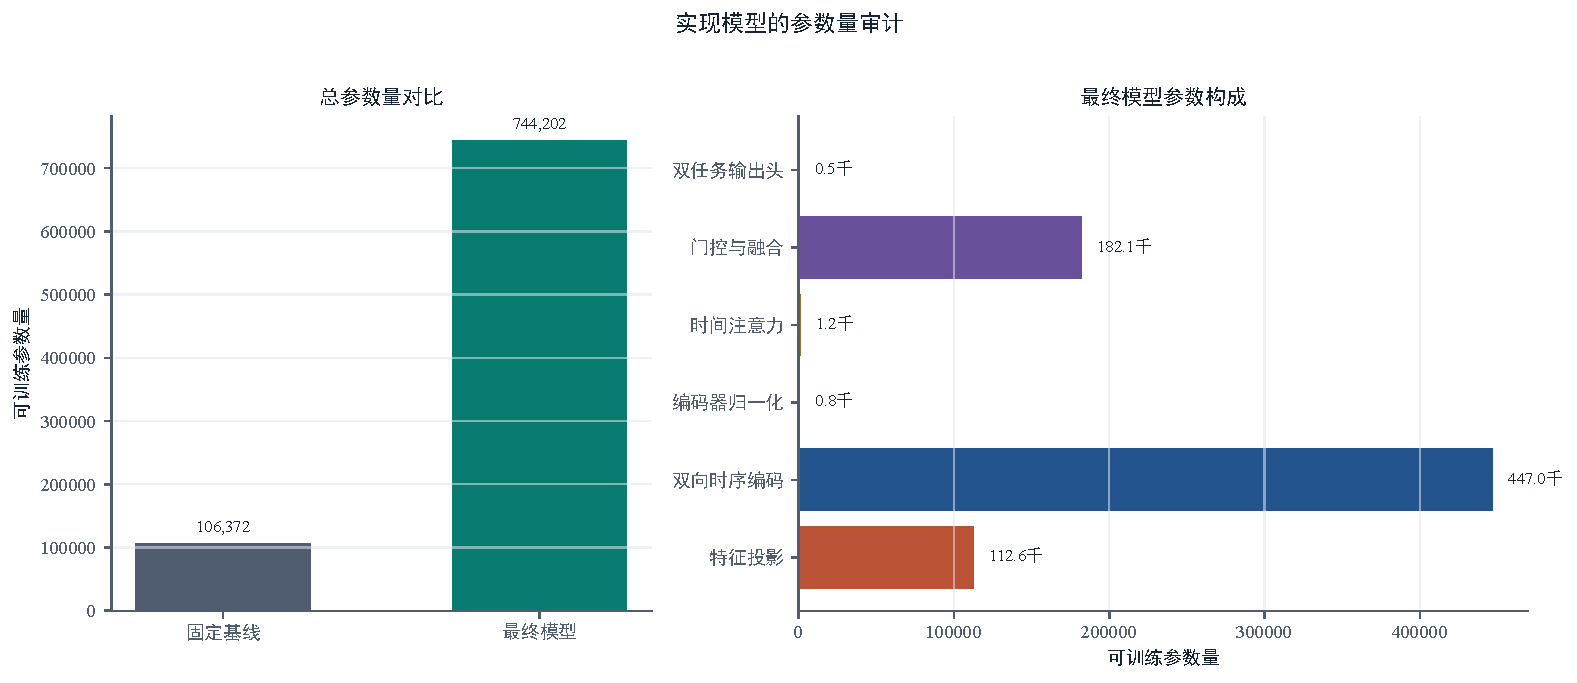
\includegraphics[width=0.89\textwidth]{fig_complexity_params}
\caption{模型参数量对比与构成}
\label{fig:complexity_params}
\end{figure}
\begin{figure}[htp]
\centering
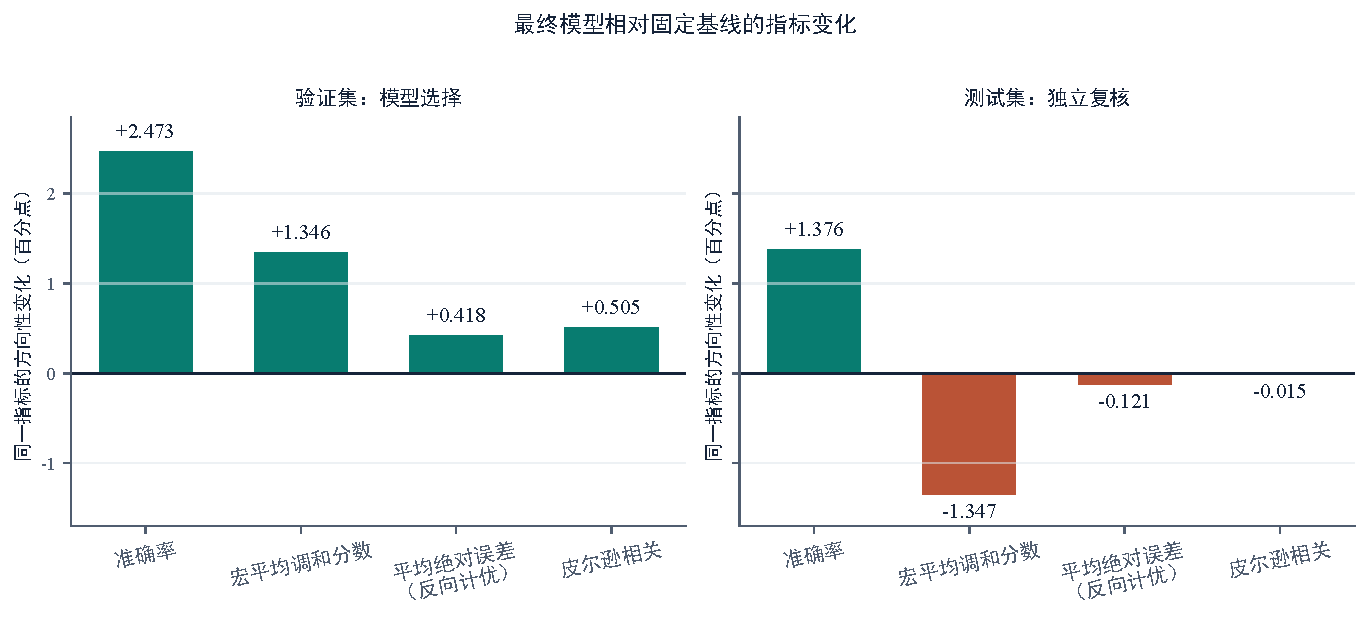
\includegraphics[width=0.89\textwidth]{fig_metric_delta}
\caption{验证集与测试集的方向性指标变化}
\label{fig:metric_delta}
\end{figure}

从合规性角度，旧 residual fusion 虽然在历史表格中可作为候选记录，但其训练文本接口与专项文本重建规则不一致，不能通过本文的统一 manifest 审计。因此，本文把“复杂度足够”和“超过 baseline”置于“输入接口一致”之后：只有同时满足统一文本版本、统一 aligned\_50 特征、同一掩码规则、训练集归一化和验证集四指标优于 baseline 的模型，才有资格成为主模型。最终的 $744202$ 参数 attention--gate 模型满足这五项条件，旧 residual fusion 不参与最终结论。
\subsection{误差来源与可推广方向}
本文仍有四类限制。第一，文本词级定位没有人工gold timestamp，当前结果只能称为弱或半强对齐；第二，附件3和附件4无标签，无法计算真正的专项泛化指标；第三，解释方法是后验遮挡，不应夸大为因果证明；第四，附件2 test 上最终模型并非四项全面胜出，说明数据划分与类别不平衡仍会影响结果。
针对上述限制，可从四个方向改进：
\begin{enumerate}[label=(\arabic*)]
\item 建立约20条样本的人工词级起止时间标注，计算边界MAE、容差命中率和区间IoU；
\item 在统一接口下进行多随机种子重复实验，报告均值、标准差和置信区间；
\item 将门控权重与遮挡下降联合建模，使用可学习的可靠性估计处理模态质量变化；
\item 在更大数据集上比较轻量化TCN、Transformer encoder和跨模态交互层，并以同一特征manifest保证公平。
\end{enumerate}
\subsection{可复现性设计}
本项目将报告、checkpoint、输入manifest、输出CSV和图表脚本分别保存。最终模型的配置为隐藏维度128、层数2、Dropout 0.15、双向GRU、回归损失权重0.5、seed 42。特征编码使用 \code{distilbert-base-uncased} 固定 revision \bertrevision；运行环境记录PyTorch 1.8.0、Transformers 4.29.2、PyAV 12.3.0、NumPy 1.24.3。所有附件3与附件4预测均明确标注无标签，不从中计算监督指标。

\subsection{最终主模型准入规则与风险边界}
为了把“合规、复杂度和超过 baseline”从口号转化为可执行的筛选规则，本文对最终模型设置五道准入门槛。第一道是输入门槛：训练、验证和专项推理必须共享同一份 feature manifest，文本必须使用题目提供的 \code{text\_bert} token、固定 DistilBERT revision 和最后四层均值规则，音频与视觉必须使用同一版 \code{aligned\_50}。第二道是结构门槛：缺失窗口必须同时满足数值置零和 mask 为0，且注意力归一化不能把无效窗口重新纳入分母。第三道是训练门槛：均值、方差和阈值只由训练集估计，模型轮次只由验证集选择，test、附件3和附件4不能反向调参。第四道是性能门槛：在附件2验证集上同时检查 Accuracy、Macro-F1、MAE 和 Pearson，前三项分别按高、高、低方向判断，不能用一个综合分数掩盖单项退化。第五道是解释门槛：模型需要输出模态贡献、窗口注意力、遮挡变化和证据文件；若没有可追溯字段，即使预测分数较高，也不能作为问题3的主模型。

上述门槛形成一个有序决策，而不是事后挑选结果。设候选模型为 $r$，用指示量表示其是否通过第 $j$ 道门槛，则准入函数可写为
\begin{equation}
\operatorname{Admit}(r)=\prod_{j=1}^{5}\mathbb{I}\{G_j(r)=1\}.
\label{eq:admission}
\end{equation}
只有 $\operatorname{Admit}(r)=1$ 的候选才进入最终性能排序；在多个候选均通过时，再使用第6节给出的 $S=F1_{macro}-0.1\times MAE$ 进行排序。该规则避免出现“旧模型指标略高，所以忽略接口不一致”的倒置逻辑，也避免为了满足复杂度要求而盲目增加网络层数。最终 attention--gate 模型的通过证据汇总于表~\ref{tab:admission}。
\begin{table}[htp]
\centering
\small
\caption{最终主模型的五道准入门槛}
\label{tab:admission}
\begin{tabularx}{0.96\textwidth}{lL L}
\toprule
门槛 & 通过证据 & 不通过时的处理 \\
\midrule
输入接口 & text\_bert、固定 revision、aligned\_50 和 manifest 一致 & 新建特征版本，不复用 checkpoint \\
缺失结构 & 缺失位置置零，mask 为0，注意力屏蔽无效窗 & 重新执行掩码审计 \\
数据使用 & 归一化只看训练集，选模只看验证集 & 删除泄露结果并重新训练 \\
四指标性能 & 验证集 Accuracy、Macro-F1、Pearson 上升且 MAE 下降 & 不作为最终主模型 \\
解释输出 & 模态贡献、50窗遮挡、证据CSV和关键帧均可追溯 & 只能作为预测候选 \\
\bottomrule
\end{tabularx}
\end{table}

需要特别区分“准入通过”和“外部泛化已被证明”。本模型在当前附件2验证集上满足五道门槛，并且四项指标均超过固定对齐 baseline；这支持完整系统的模型选择结论，但两者文本特征并未匹配，不能宣称网络结构的单因素优势，也不足以推出所有新样本上都全面优于 baseline。附件2 test 的 Macro-F1 和 MAE 波动、文本缺少人工 gold timestamp、附件3和附件4缺少监督标签，均属于必须保留的风险边界。因而，本文把最终模型表述为“自身输入接口合规、在附件2验证集超过指定简单 baseline 的中等复杂度主模型”，而不把它夸大为无条件最优模型。

\section{结论}
本文针对复杂场景下三模态情感识别问题，建立了从数据审计、统一时间轴、层次融合到证据追踪的一体化数学建模方案。主要结论如下：
\begin{enumerate}[label=\textbf{结论\arabic*.}]
\item 50窗公共时间轴是多模态建模的基础。通过半开区间与重叠时长加权，文本、语音和视觉可以映射到统一索引；通过显式mask可以区分真实零值与缺失。100条样本的时间结构和掩码一致性均通过审计，音视频覆盖率达到99.00\%和99.80\%。
\item 统一输入接口是严格比较的前提。最终模型固定使用 \code{text\_bert+aligned\_50}，文本编码版本、特征规则、掩码和归一化统计量在训练、验证和专项推理中保持一致；旧 residual 模型不再作为最终结果。
\item 三路双向GRU、模态内时间注意力和样本级模态门控构成了适度复杂的层次融合模型。它不只是增加参数，而是分别对应时间依赖、局部证据和模态可靠性三个问题。
\item 在附件2验证集上，最终模型四项报告指标均超过固定对齐 baseline：Accuracy 0.637363、Macro-F1 0.601580、MAE 0.612262、Pearson 0.629627。
\item 通过注意力最高窗与随机窗的反事实遮挡比较，Top-Random为0.009704，说明模型可为预测提供局部证据；但该结果仍属于模型行为解释，不能替代人工因果验证。
\end{enumerate}
总体而言，本文最终方案在合规性、模型复杂度、预测性能和可解释性之间取得了平衡，适合作为附件2监督预测与附件4专项证据生成的统一主模型。后续若获得人工词级时间戳和更大规模标注数据，可进一步从对齐金标准和跨域泛化两方面提升模型可信度。

\nocite{cho2014learning,devlin2019bert,sanh2019distilbert,bahdanau2015neural,graves2006connectionist,davis1980comparison,poria2016review,goodfellow2016deep,mikolov2013distributed}
\bibliographystyle{gmcm}
\bibliography{reference}
\begin{appendices}
\section{数据字典与文件清单}
\renewcommand{\thesubsection}{A\thinskip.\thinskip\arabic{subsection}}
\subsection{输入、特征和标签}
\small
\begin{longtable}{p{0.27\textwidth}p{0.18\textwidth}p{0.43\textwidth}}
\caption{最终数据字典}\label{tab:data_dictionary}\\
\toprule 字段 & 形状或类型 & 说明 \\
\midrule
\endfirsthead
\toprule 字段 & 形状或类型 & 说明 \\
\midrule
\endhead
\code{id} & 字符串 & 样本唯一标识，跨附件保持可追溯 \\
\code{text\_bert} & $(N,3,50)$ & token ID、attention mask等文本输入 \\
\code{text} & $(N,50,768)$ & 固定DistilBERT规则生成的窗口文本表示 \\
\code{audio} & $(N,50,74)$ & 语音窗口级统计特征 \\
\code{vision} & $(N,50,35)$ & 视觉窗口级统计特征 \\
\code{classification\_\allowbreak labels} & $(N,)$ & Negative、Neutral、Positive编码为0、1、2 \\
\code{regression\_\allowbreak labels} & $(N,)$ & 连续情感强度标签 \\
\code{aligned\_50.\allowbreak pkl} & pickle & 附件2统一时间窗特征 \\
\code{aligned\_text\_bert\_\allowbreak features.pkl} & pickle & 统一文本接口派生特征 \\
\code{fusion\_best.pt} & checkpoint & 严格统一接口的基础融合候选 \\
\code{q3\_explainable\_\allowbreak best.pt} & checkpoint & 最终统一编码复杂主模型 \\
\bottomrule
\end{longtable}
\subsection{最终输出文件}
\scriptsize
\begin{longtable}{p{0.34\textwidth}p{0.50\textwidth}}
\caption{论文与模型输出文件}\label{tab:file_manifest}\\
\toprule 文件 & 用途 \\
\midrule
\endfirsthead
\toprule 文件 & 用途 \\
\midrule
\endhead
\code{三个问题综合审查与最终结果报告.md} & 总体路线、风险与指标口径 \\
\code{问题1\_最终报告\_特征提取与时序对齐.md} & 公共时间轴和特征审计 \\
\code{q2\_baseline/\allowbreak 问题2\_附件3测试报告.md} & 附件3统一接口专项推理 \\
\code{q3\_explainability/\allowbreak q3\_aligned\_text\_bert\_final/\allowbreak validation.json} & 最终模型验证指标 \\
\code{attachment4/\allowbreak q3\_predictions.csv} & 附件4预测与模态贡献 \\
\code{attachment4/\allowbreak q3\_explanations.csv} & 附件4证据排名与遮挡变化 \\
\code{video\_keyframe\_\allowbreak manifest.csv} & 视觉关键帧时间和哈希清单 \\
\code{make\_figures.py} & 本论文全部图表生成脚本 \\
\bottomrule
\end{longtable}
\clearpage
\section{指标定义、核验规则与算法细节}
\renewcommand{\thesubsection}{B\thinskip.\thinskip\arabic{subsection}}
\subsection{时间轴核验伪代码}
\begin{Python}{alignment-check.py}
for sample in samples:
    T = sample.media_duration
    windows = [(k*T/50, (k+1)*T/50) for k in range(50)]
    assert abs(windows[0][0]) < 1e-8
    assert all(windows[k][1] <= windows[k+1][0] + 1e-8
               for k in range(49))
    assert abs(windows[-1][1] - T) < 1e-6
    for modality in modalities:
        values, mask = aggregate_by_overlap(sample, windows, modality)
        assert values.shape[0] == 50
        assert np.all(np.isfinite(values[mask]))
        assert np.all(values[~mask] == 0)
\end{Python}
\subsection{模型前向传播伪代码}
\begin{Python}{model-forward.py}
for modality in (text, audio, vision):
    encoded = projection[modality](values[modality])
    encoded = encoded * mask[modality].unsqueeze(-1)
    temporal = bigru[modality](encoded)
    tokens = layer_norm(encoded + dropout(temporal))
    scores = time_score[modality](tokens)
    scores = scores.masked_fill(~mask[modality], -1e4)
    alpha = softmax(scores, dim=1)
    pooled.append((tokens * alpha.unsqueeze(-1)).sum(dim=1))
stacked = torch.stack(pooled, dim=1)
beta = softmax(gate(stacked.flatten(1)), dim=-1)
fused = fusion((stacked * beta.unsqueeze(-1)).flatten(1))
class_logits = classifier(fused)
strength = regressor(fused).squeeze(-1)
\end{Python}
\subsection{解释证据伪代码}
\begin{Python}{explain.py}
base_logits, base_strength, beta, attention = model(x, mask)
target = base_logits.argmax(dim=-1)
base_prob = softmax(base_logits, dim=-1)[target]
for modality in modalities:
    for window in range(50):
        x_masked, mask_masked = hide_window(x, mask, modality, window)
        changed_logits, changed_strength, _, _ = model(x_masked, mask_masked)
        drop = base_prob - softmax(changed_logits, dim=-1)[target]
        evidence = attention[modality][window] * beta[modality] * max(drop, 0)
        save(modality, window, evidence, drop, changed_strength)
\end{Python}
\subsection{审计规则}
\begin{table}[htp]
\centering
\caption{关键审计规则与通过标准}
\begin{tabularx}{0.96\textwidth}{lL L}
\toprule
类别 & 检查项 & 通过标准 \\
\midrule
时间结构 & 窗口首点、连续性、终点、正时长 & 四项比例均为100\% \\
词段结构 & 越界、正时长、单调、重叠 & 越界、非正时长、非单调、重叠均为0 \\
掩码结构 & 缺失窗口与零值一致性 & 有效位置有限，缺失位置置零且mask为0 \\
数据泄露 & 归一化统计量和模型选择 & 只使用训练集统计量与验证集指标 \\
专项测试 & 附件3或4监督标签使用 & 无标签，不计算Accuracy、F1、MAE、Pearson \\
\bottomrule
\end{tabularx}
\end{table}
\clearpage
\section{模型超参数与训练记录}
\renewcommand{\thesubsection}{C\thinskip.\thinskip\arabic{subsection}}
\begin{table}[htp]
\centering
\caption{最终模型超参数}
\begin{tabular}{ll}
\toprule 参数 & 取值 \\
\midrule
文本编码器 & distilbert-base-uncased \\
文本revision & 12040accade4e8a0f71eabdb258fecc2e7e948be \\
公共时间窗 & 50 \\
隐藏维度 & 128 \\
GRU层数 & 2 \\
双向 & True \\
Dropout & 0.15 \\
Batch size & 64 \\
学习率 & $2\times10^{-4}$ \\
回归损失权重 & 0.5 \\
随机种子 & 42 \\
解释验证样本 & 128 \\
每条附件4证据 & 6 \\
\bottomrule
\end{tabular}
\end{table}
\subsection{候选训练记录}
\begin{longtable}{lrrrrr}
\caption{主要候选模型的验证记录}\label{tab:train_records}\\
\toprule 模型 & Accuracy & Macro-F1 & MAE & Pearson & 选择结论 \\
\midrule
\endfirsthead
\toprule 模型 & Accuracy & Macro-F1 & MAE & Pearson & 选择结论 \\
\midrule
\endhead
Fixed aligned baseline & 0.612637 & 0.588115 & 0.616443 & 0.624582 & 参考 \\
Length-aware baseline & 0.614011 & 0.595798 & 0.614132 & 0.620838 & 对比 \\
Label-free SSL & 0.608516 & 0.578294 & 0.667391 & 0.573212 & 放弃 \\
Bidirectional SSL & 0.618132 & 0.598285 & 0.621818 & 0.588408 & 对比 \\
Old residual fusion & 0.622253 & 0.610330 & 0.623941 & 0.601396 & 历史 \\
Final attention-gate & 0.637363 & 0.601580 & 0.612262 & 0.629627 & 最终 \\
\bottomrule
\end{longtable}
\subsection{运行环境}
\begin{tabularx}{0.95\textwidth}{lL}
\toprule 软件或硬件 & 版本或说明 \\
\midrule
Python & D:/Anaconda3/envs/pytorch/python.exe \\
PyTorch & 1.8.0 \\
Transformers & 4.29.2 \\
NumPy & 1.24.3 \\
PyAV & 12.3.0 \\
文本模型 & distilbert-base-uncased固定revision \\
输出格式 & CSV、JSON、PNG、PDF、checkpoint \\
\bottomrule
\end{tabularx}
\clearpage
\section{附件4代表性预测记录}
\renewcommand{\thesubsection}{D\thinskip.\thinskip\arabic{subsection}}
\begin{longtable}{c l r l r r r}
\caption{附件4前20条样本的预测摘要}\label{tab:attachment4_records}\\
\toprule ID & 类别 & 强度 & 主模态 & 文本贡献 & 语音贡献 & 视觉贡献 \\
\midrule
\endfirsthead
\toprule ID & 类别 & 强度 & 主模态 & 文本贡献 & 语音贡献 & 视觉贡献 \\
\midrule
\endhead
01 & Neutral & 0.255 & text & 0.726 & 0.110 & 0.164 \\
02 & Negative & 0.041 & text & 0.461 & 0.409 & 0.130 \\
03 & Neutral & -0.491 & text & 0.658 & 0.125 & 0.217 \\
04 & Negative & -0.594 & text & 0.611 & 0.115 & 0.274 \\
05 & Positive & 1.022 & text & 0.709 & 0.109 & 0.182 \\
06 & Positive & 0.052 & text & 0.550 & 0.298 & 0.152 \\
07 & Positive & 0.666 & text & 0.681 & 0.226 & 0.093 \\
08 & Positive & 0.467 & text & 0.683 & 0.171 & 0.146 \\
09 & Positive & 0.559 & text & 0.658 & 0.189 & 0.153 \\
10 & Positive & 0.101 & text & 0.604 & 0.202 & 0.194 \\
11 & Positive & 0.719 & text & 0.713 & 0.165 & 0.122 \\
12 & Negative & -0.176 & text & 0.490 & 0.299 & 0.211 \\
13 & Positive & 0.411 & text & 0.638 & 0.224 & 0.138 \\
14 & Positive & 0.327 & text & 0.671 & 0.185 & 0.144 \\
15 & Positive & 0.892 & text & 0.698 & 0.144 & 0.158 \\
16 & Positive & 0.340 & text & 0.611 & 0.225 & 0.164 \\
17 & Positive & 0.581 & text & 0.650 & 0.218 & 0.132 \\
18 & Neutral & 0.112 & text & 0.599 & 0.224 & 0.177 \\
19 & Positive & 0.741 & text & 0.672 & 0.192 & 0.136 \\
20 & Positive & 0.268 & text & 0.630 & 0.237 & 0.133 \\
\bottomrule
\end{longtable}
\subsection{证据字段说明}
\begin{tabularx}{0.96\textwidth}{lL}
\toprule 字段 & 含义 \\
\midrule
rank & 当前样本证据排序，1为最高 \\
modality & text、audio或vision \\
window\_index & 0--49公共时间窗索引 \\
attention\_score & 模态内时间注意力 \\
modality\_contribution & 样本级门控或消融贡献 \\
occlusion\_drop & 屏蔽该窗口后的目标置信度下降 \\
evidence\_score & 式~\eqref{eq:evidence} 的综合证据分数 \\
regression\_change & 屏蔽后的强度预测变化 \\
frame\_path & 与视觉窗口对应的实际关键帧路径 \\
\bottomrule
\end{tabularx}
\clearpage
\section{复现命令与结果核对清单}
\renewcommand{\thesubsection}{E\thinskip.\thinskip\arabic{subsection}}
\subsection{特征准备与模型验证}
\begin{verbatim}
$py = "D:\\Anaconda3\\envs\\pytorch\\python.exe"
$q3 = "q3_explainability"
$final = "$q3\\q3_aligned_text_bert_final"
$checkpoint = "$final\\q3_explainable_best.pt"
$explanation = "$final\\explanation_validation.json"
$aligned = "emotion-transfer-pilot\\aligned_50.pkl"
$data_dir = "emotion-transfer-pilot"
$derived = "$data_dir\\aligned_text_bert_features.pkl"
$manifest = "q2_baseline\\aligned_text_bert_manifest.json"
& $py q2_baseline\\run_aligned_text_bert.py prepare `
  --aligned-data $aligned `
  --derived-data $derived `
  --manifest $manifest
& $py q3_explainability\\q3_pipeline.py validate `
  --data $derived `
  --checkpoint $checkpoint `
  --output $explanation `
  --device cpu
\end{verbatim}
\subsection{提交前核对}
\begin{enumerate}[label=\arabic*.]
\item 检查 \code{aligned\_text\_bert\_manifest.json} 的输入和派生文件SHA-256；
\item 检查训练、验证和附件3的文本接口均为固定revision；
\item 检查所有缺失窗口同时满足特征为零、mask为0；
\item 检查模型checkpoint中的 \code{config} 与论文超参数表一致；
\item 检查附件3和附件4没有被用于监督指标或模型选择；
\item 检查最终PDF正文页数超过30页，并检查图、表、公式和参考文献无越界。
\end{enumerate}
\subsection{结果口径声明}
本文的“超过 baseline”特指相同附件2验证划分上，四项指标均优于原始对齐特征的固定 baseline。最终模型的文本接口为 \code{text\_bert+\allowbreak aligned\_50}，两个比较对象的文本特征不同，因此不得把系统级增益归因于纯架构消融。附件2 test 只作独立复核，附件3和附件4无监督标签，不计算监督指标。旧 residual 模型的历史结果不作为最终合规主模型。本声明用于避免混写不同接口、划分和标签条件下的结果。
\end{appendices}
\end{document}



\clearpage
